%% LyX 2.3.7 created this file.  For more info, see http://www.lyx.org/.
%% Do not edit unless you really know what you are doing.
\documentclass[journal,article,submit,pdftex,moreauthors]{Definitions/mdpi}
\usepackage[utf8]{inputenc}
\usepackage{float}
\usepackage{url}
\usepackage{graphicx}

\makeatletter

%%%%%%%%%%%%%%%%%%%%%%%%%%%%%% LyX specific LaTeX commands.

\Title{RbfCon: Construct RBF neural networks with Grammatical Evolution}

\TitleCitation{RbfCon: Construct RBF neural networks with Grammatical Evolution}

\Author{Ioannis G. Tsoulos$^{1,*}$, Ioannis Varvaras$^{2}$ and Vasileios
Charilogis$^{3}$}

\AuthorNames{Ioannis G. Tsoulos, Ioannis Varvaras and Vasileios Charilogis }

\AuthorCitation{Tsoulos, I.G.; Varvaras, I.; Charilogis, V. }


\address{$^{1}$\quad{}Department of Informatics and Telecommunications,
University of Ioannina, Greece; itsoulos@uoi.gr\\
$^{2}$\quad{}Department of Informatics and Telecommunications, University
of Ioannina, Greece; i\_varvaras@hotmail.com\\
$^{3}\quad$Department of Informatics and Telecommunications, University
of Ioannina, Greece; v.charilog@uoi.gr}


\corres{Correspondence: itsoulos@uoi.gr}


\abstract{Radial Basis Function networks considered as a machine learning tool,
applied on a wide series of classification and regression problems
that was proposed in various research topics of the modern world.
However, in many cases, the initial training method used to fit the
parameters of these models can produce poor results either due to
unstable numerical operations or its inability to effectively locate
the lowest value of the error function. The current work proposes
a novel method that constructs the architecture of this model and
estimates the values for each parameter of the model with the incorporation
of Grammatical Evolution. The proposed method was coded in ANSI C++
and the produced software was tested for its effectiveness on a wide
series of datasets. The experimental results certify the adequacy
of the new method to solve difficult problems and in the vast majority
of cases the error in classification or approximation of functions
is significantly lower than the case where the original training method
was applied.}


\keyword{Neural networks; Genetic programming; Grammatical Evolution; Evolutionary
algorithms}

\DeclareTextSymbolDefault{\textquotedbl}{T1}
%% Because html converters don't know tabularnewline
\providecommand{\tabularnewline}{\\}
\floatstyle{ruled}
\newfloat{algorithm}{tbp}{loa}
\providecommand{\algorithmname}{Algorithm}
\floatname{algorithm}{\protect\algorithmname}

%%%%%%%%%%%%%%%%%%%%%%%%%%%%%% Textclass specific LaTeX commands.
\newenvironment{lyxcode}
	{\par\begin{list}{}{
		\setlength{\rightmargin}{\leftmargin}
		\setlength{\listparindent}{0pt}% needed for AMS classes
		\raggedright
		\setlength{\itemsep}{0pt}
		\setlength{\parsep}{0pt}
		\normalfont\ttfamily}%
	 \item[]}
	{\end{list}}

%%%%%%%%%%%%%%%%%%%%%%%%%%%%%% User specified LaTeX commands.
%  LaTeX support: latex@mdpi.com 
%  For support, please attach all files needed for compiling as well as the log file, and specify your operating system, LaTeX version, and LaTeX editor.

%=================================================================


% For posting an early version of this manuscript as a preprint, you may use "preprints" as the journal and change "submit" to "accept". The document class line would be, e.g., \documentclass[preprints,article,accept,moreauthors,pdftex]{mdpi}. This is especially recommended for submission to arXiv, where line numbers should be removed before posting. For preprints.org, the editorial staff will make this change immediately prior to posting.

%--------------------
% Class Options:
%--------------------
%----------
% journal
%----------
% Choose between the following MDPI journals:
% acoustics, actuators, addictions, admsci, adolescents, aerospace, agriculture, agriengineering, agronomy, ai, algorithms, allergies, alloys, analytica, animals, antibiotics, antibodies, antioxidants, applbiosci, appliedchem, appliedmath, applmech, applmicrobiol, applnano, applsci, aquacj, architecture, arts, asc, asi, astronomy, atmosphere, atoms, audiolres, automation, axioms, bacteria, batteries, bdcc, behavsci, beverages, biochem, bioengineering, biologics, biology, biomass, biomechanics, biomed, biomedicines, biomedinformatics, biomimetics, biomolecules, biophysica, biosensors, biotech, birds, bloods, blsf, brainsci, breath, buildings, businesses, cancers, carbon, cardiogenetics, catalysts, cells, ceramics, challenges, chemengineering, chemistry, chemosensors, chemproc, children, chips, cimb, civileng, cleantechnol, climate, clinpract, clockssleep, cmd, coasts, coatings, colloids, colorants, commodities, compounds, computation, computers, condensedmatter, conservation, constrmater, cosmetics, covid, crops, cryptography, crystals, csmf, ctn, curroncol, currophthalmol, cyber, dairy, data, dentistry, dermato, dermatopathology, designs, diabetology, diagnostics, dietetics, digital, disabilities, diseases, diversity, dna, drones, dynamics, earth, ebj, ecologies, econometrics, economies, education, ejihpe, electricity, electrochem, electronicmat, electronics, encyclopedia, endocrines, energies, eng, engproc, ent, entomology, entropy, environments, environsciproc, epidemiologia, epigenomes, est, fermentation, fibers, fintech, fire, fishes, fluids, foods, forecasting, forensicsci, forests, foundations, fractalfract, fuels, futureinternet, futureparasites, futurepharmacol, futurephys, futuretransp, galaxies, games, gases, gastroent, gastrointestdisord, gels, genealogy, genes, geographies, geohazards, geomatics, geosciences, geotechnics, geriatrics, hazardousmatters, healthcare, hearts, hemato, heritage, highthroughput, histories, horticulturae, humanities, humans, hydrobiology, hydrogen, hydrology, hygiene, idr, ijerph, ijfs, ijgi, ijms, ijns, ijtm, ijtpp, immuno, informatics, information, infrastructures, inorganics, insects, instruments, inventions, iot, j, jal, jcdd, jcm, jcp, jcs, jdb, jeta, jfb, jfmk, jimaging, jintelligence, jlpea, jmmp, jmp, jmse, jne, jnt, jof, joitmc, jor, journalmedia, jox, jpm, jrfm, jsan, jtaer, jzbg, kidney, kidneydial, knowledge, land, languages, laws, life, liquids, literature, livers, logics, logistics, lubricants, lymphatics, machines, macromol, magnetism, magnetochemistry, make, marinedrugs, materials, materproc, mathematics, mca, measurements, medicina, medicines, medsci, membranes, merits, metabolites, metals, meteorology, methane, metrology, micro, microarrays, microbiolres, micromachines, microorganisms, microplastics, minerals, mining, modelling, molbank, molecules, mps, msf, mti, muscles, nanoenergyadv, nanomanufacturing, nanomaterials, ncrna, network, neuroglia, neurolint, neurosci, nitrogen, notspecified, nri, nursrep, nutraceuticals, nutrients, obesities, oceans, ohbm, onco, oncopathology, optics, oral, organics, organoids, osteology, oxygen, parasites, parasitologia, particles, pathogens, pathophysiology, pediatrrep, pharmaceuticals, pharmaceutics, pharmacoepidemiology, pharmacy, philosophies, photochem, photonics, phycology, physchem, physics, physiologia, plants, plasma, pollutants, polymers, polysaccharides, poultry, powders, preprints, proceedings, processes, prosthesis, proteomes, psf, psych, psychiatryint, psychoactives, publications, quantumrep, quaternary, qubs, radiation, reactions, recycling, regeneration, religions, remotesensing, reports, reprodmed, resources, rheumato, risks, robotics, ruminants, safety, sci, scipharm, seeds, sensors, separations, sexes, signals, sinusitis, skins, smartcities, sna, societies, socsci, software, soilsystems, solar, solids, sports, standards, stats, stresses, surfaces, surgeries, suschem, sustainability, symmetry, synbio, systems, taxonomy, technologies, telecom, test, textiles, thalassrep, thermo, tomography, tourismhosp, toxics, toxins, transplantology, transportation, traumacare, traumas, tropicalmed, universe, urbansci, uro, vaccines, vehicles, venereology, vetsci, vibration, viruses, vision, waste, water, wem, wevj, wind, women, world, youth, zoonoticdis 

%---------
% article
%---------
% The default type of manuscript is "article", but can be replaced by: 
% abstract, addendum, article, book, bookreview, briefreport, casereport, comment, commentary, communication, conferenceproceedings, correction, conferencereport, entry, expressionofconcern, extendedabstract, datadescriptor, editorial, essay, erratum, hypothesis, interestingimage, obituary, opinion, projectreport, reply, retraction, review, perspective, protocol, shortnote, studyprotocol, systematicreview, supfile, technicalnote, viewpoint, guidelines, registeredreport, tutorial
% supfile = supplementary materials

%----------
% submit
%----------
% The class option "submit" will be changed to "accept" by the Editorial Office when the paper is accepted. This will only make changes to the frontpage (e.g., the logo of the journal will get visible), the headings, and the copyright information. Also, line numbering will be removed. Journal info and pagination for accepted papers will also be assigned by the Editorial Office.

%------------------
% moreauthors
%------------------
% If there is only one author the class option oneauthor should be used. Otherwise use the class option moreauthors.

%---------
% pdftex
%---------
% The option pdftex is for use with pdfLaTeX. If eps figures are used, remove the option pdftex and use LaTeX and dvi2pdf.

%=================================================================
% MDPI internal commands - do not modify
\firstpage{1} 
 
\setcounter{page}{\@firstpage} 

\pubvolume{1}
\issuenum{1}
\articlenumber{0}
\pubyear{2024}
\copyrightyear{2024}
%\externaleditor{Academic Editor: Firstname Lastname} % For journal Automation, please change Academic Editor to "Communicated by"
\datereceived{}
\daterevised{ } % Comment out if no revised date
\dateaccepted{}
\datepublished{}
%\datecorrected{} % Corrected papers include a "Corrected: XXX" date in the original paper.
%\dateretracted{} % Corrected papers include a "Retracted: XXX" date in the original paper.
\hreflink{https://doi.org/} % If needed use \linebreak
%\doinum{}
%------------------------------------------------------------------
% The following line should be uncommented if the LaTeX file is uploaded to arXiv.org
%\pdfoutput=1

%=================================================================
% Add packages and commands here. The following packages are loaded in our class file: fontenc, inputenc, calc, indentfirst, fancyhdr, graphicx, epstopdf, lastpage, ifthen, lineno, float, amsmath, setspace, enumitem, mathpazo, booktabs, titlesec, etoolbox, tabto, xcolor, soul, multirow, microtype, tikz, totcount, changepage, attrib, upgreek, cleveref, amsthm, hyphenat, natbib, hyperref, footmisc, url, geometry, newfloat, caption

%=================================================================
%% Please use the following mathematics environments: Theorem, Lemma, Corollary, Proposition, Characterization, Property, Problem, Example, ExamplesandDefinitions, Hypothesis, Remark, Definition, Notation, Assumption
%% For proofs, please use the proof environment (the amsthm package is loaded by the MDPI class).

%=================================================================
% The fields PACS, MSC, and JEL may be left empty or commented out if not applicable
%\PACS{J0101}
%\MSC{}
%\JEL{}

%%%%%%%%%%%%%%%%%%%%%%%%%%%%%%%%%%%%%%%%%%
% Only for the journal Diversity
%\LSID{\url{http://}}

%%%%%%%%%%%%%%%%%%%%%%%%%%%%%%%%%%%%%%%%%%
% Only for the journal Applied Sciences:
%\featuredapplication{Authors are encouraged to provide a concise description of the specific application or a potential application of the work. This section is not mandatory.}
%%%%%%%%%%%%%%%%%%%%%%%%%%%%%%%%%%%%%%%%%%

%%%%%%%%%%%%%%%%%%%%%%%%%%%%%%%%%%%%%%%%%%
% Only for the journal Data:
%\dataset{DOI number or link to the deposited data set in cases where the data set is published or set to be published separately. If the data set is submitted and will be published as a supplement to this paper in the journal Data, this field will be filled by the editors of the journal. In this case, please make sure to submit the data set as a supplement when entering your manuscript into our manuscript editorial system.}

%\datasetlicense{license under which the data set is made available (CC0, CC-BY, CC-BY-SA, CC-BY-NC, etc.)}

%%%%%%%%%%%%%%%%%%%%%%%%%%%%%%%%%%%%%%%%%%
% Only for the journal Toxins
%\keycontribution{The breakthroughs or highlights of the manuscript. Authors can write one or two sentences to describe the most important part of the paper.}

%%%%%%%%%%%%%%%%%%%%%%%%%%%%%%%%%%%%%%%%%%
% Only for the journal Encyclopedia
%\encyclopediadef{Instead of the abstract}
%\entrylink{The Link to this entry published on the encyclopedia platform.}
%%%%%%%%%%%%%%%%%%%%%%%%%%%%%%%%%%%%%%%%%%

%%%%%%%%%%%%%%%%%%%%%%%%%%%%%%%%%%%%%%%%%%
% Only for the journal Advances in Respiratory Medicine
%\addhighlights{yes}
%\renewcommand{\addhighlights}{%

%\noindent This is an obligatory section in “Advances in Respiratory Medicine”, whose goal is to increase the discoverability and readability of the article via search engines and other scholars. Highlights should not be a copy of the abstract, but a simple text allowing the reader to quickly and simplified find out what the article is about and what can be cited from it. Each of these parts should be devoted up to 2~bullet points.\vspace{3pt}\\
%\textbf{What are the main findings?}
% \begin{itemize}[labelsep=2.5mm,topsep=-3pt]
% \item First bullet.
% \item Second bullet.
% \end{itemize}\vspace{3pt}
%\textbf{What is the implication of the main finding?}
% \begin{itemize}[labelsep=2.5mm,topsep=-3pt]
% \item First bullet.
% \item Second bullet.
% \end{itemize}
%}
%%%%%%%%%%%%%%%%%%%%%%%%%%%%%%%%%%%%%%%%%%

\makeatother

\usepackage{listings}
\renewcommand{\lstlistingname}{\inputencoding{latin9}Listing}

\begin{document}
\maketitle

\section{Introduction}

A variety of real - world problems can be considered as classification
and regression problems, handled by machine learning models that have
been thoroughly studied in the recent bibliography. Such problems
arise in physics \citep{physics-ml1,physics_ml2}, chemistry \citep{chemistry_ml1,chemistry_ml2},
economics \citep{econ_ml1,econ_ml2}, medicine \citep{med_ml1,med_ml2}
etc. One common machine learning model, that is applied in many areas,
is the Radial Basis Function (RBF) neural network \citep{rbf1,rbf2}.
Commonly these neural networks are formed using the following mathematical
expression:\textbf{
\begin{equation}
y\left(\overrightarrow{x}\right)=\sum_{i=1}^{k}w_{i}\phi\left(\left\Vert \overrightarrow{x}-\overrightarrow{c_{i}}\right\Vert \right)\label{eq:firstrbf}
\end{equation}
}The following notation is used in Equation \ref{eq:firstrbf}:
\begin{enumerate}
\item The vector $\overrightarrow{x}$ represents the input pattern with
dimension $d$.
\item The parameter $k$ stands for the number of weights of the model.
These weights are represented by vector $\overrightarrow{w}$
\item The vectors $\overrightarrow{c_{i}},\ i=1,..,k$ represent the so
- called centers of the network.
\item The final output of the model for the input pattern $\overrightarrow{x}$
is denoted by $y\left(\overrightarrow{x}\right)$
\item The function $\phi(x)$ in most cases is represented by the Gaussian
function defined as:\textbf{ 
\begin{equation}
\phi(x)=\exp\left(-\frac{\left(x-c\right)^{2}}{\sigma^{2}}\right)
\end{equation}
}This function is selected as the output function, since the output
value $\phi(x)$ uses only the distance of vectors $x$ and $c$.
\end{enumerate}
RBF neural networks have been extensively used and studied in the
recent literature and, among others, one can find applications in
problems derived from physics \citep{rbfphysics1,rbfphysics2}, robotics
\citep{rbfrobotics1,rbfrobotics2}, security problems \citep{rbf_dos1,rbf_dos2},
image processing \citep{rbf_lmage1,rbf_image2} etc. Due to the widespread
use of these machine learning models and their use in both classification
and data fitting problems, a number of techniques have been presented
in recent years that seek to more accurately identify their parameters.
Such methods include techniques used to initialize the parameters
of these models \citep{rbfinit1,rbfinit2,rbfinit3}, or pruning methods
for the optimal adaptation of the architecture of these models \citep{rbfprun1,rbfprun3,rbfprun2}.
Also, global optimization methods have been proposed to estimate the
optimal set of parameters of RBF networks in a series of research
papers \citep{rbf_go1,rbf_go2,rbf_go3}. 

Furthermore, a discussion on the kernel widths of RBF networks is
provided in the work of Benoudjit et al \citep{rbfkernel}. Paetz
proposed a method \citep{rbfgen} that can reduce the number of neurons
in RBF networks with dynamic decay adjustment, in order to increase
the generalization abilities of these networks. Yu et al. in their
work \citep{rbfcon} proposed an incremental design technique for
RBF networks in order to estimate the optimal architecture of these
networks. Moreover, Alexandridis et al. \citep{rbfpso} proposed the
incorporation of the Particle Swarm Optimization method to effectively
estimate the weights of RBF networks. Also, Neruda et al \citep{rbflearn}
provided a detailed comparison of methods used to estimate the parameters
of RBF networks. Additionally, due to the widespread usage of parallel
programming techniques, a series of techniques that exploit parallel
computing units have been suggested in recent years for RBF network
training\textbf{ }\citep{rbfpar1,rbfpar2}.

In most cases, the set of the parameters of the model is estimated
using a two phase method: during the first phase, the set of centers
and variances of equation \ref{eq:firstrbf} are calculated using
the K-Means algorithm \citep{kmeans}. In the second phase, the set
of weights $\overrightarrow{w}$ is obtained by solving a linear system
of equations. Although the previous procedure is capable of estimating
the optimal set of parameters in a very short time, it nevertheless
has a number of problems such as numerical stability, accurate determination
of the number of weights, over - fitting problems, etc. To calculate
these parameters with the classical calculation method, it is necessary
to solve a system of equations, but in many cases the solution of
such a system leads to numerical problems as determinants appear with
a value quite close to zero. To tackle such problems, a novel method
is proposed here that constructs the optimal architecture of RBF networks
using a method that incorporates the Grammatical Evolution procedure
\citep{geMain}. The proposed technique is able to estimate both the
optimal architecture of the neural network and the numerical values
of its parameters, and in this paper both the algorithm used and the
software created for this process, which is freely available from
the internet, will be presented in detail. 

The software proposed in this work is fully implemented in the programming
language ANSI C++ and is an executable that has a series of command
line parameters with which the user can efficiently process the data
sets at his disposal.\textbf{ }The contribution of the proposed technique
and the implemented software can be summarized as follows: 
\begin{enumerate}
\item The method can efficiently construct the structure of RBF networks
and achieve optimal adjustment of their parameters. 
\item The resulting networks do not have the numerical problems caused by
the traditional training technique of RBF networks. 
\item The created software provides an easy user interface for performing
experiments and can be installed on almost any operating system. 
\end{enumerate}
The rest of this article is divided in the following sections: in
section \ref{sec:Materials-and-Methods} the proposed methodology
and the used software are thoroughly discussed, in section \ref{sec:Results}
the datasets incorporated in the conducted experiments are listed
followed by the experimental results, in section \ref{sec:Discussion}
a discussion on the experimental results is provided and finally in
section \ref{sec:Conclusions} a series of conclusions is presented.

\section{Materials and Methods\label{sec:Materials-and-Methods}}

The original training method of RBF networks is presented here followed
by the detail presentation of the Grammatical Evolution procedure.
Afterwards, the proposed method is fully described accompanied by
a full working example of the proposed software.

\subsection{The original training procedure of RBF neural networks\label{subsec:The-original-training}}

The typical training procedure of an RBF network $y(x)=\sum_{i=1}^{k}w_{i}\phi\left(\left\Vert x-c_{i}\right\Vert \right)$
involves two major steps: in first step the centers $\overrightarrow{c_{i}}$
and the variances are calculated using the K-means procedure, which
is outlined in Algorithm \ref{alg:K-means-Algorithm}. During the
second step a system of equations should be solved in order to calculate
the values for weights $w_{i},\ i=1,\ldots,k$ as follows:
\begin{enumerate}
\item \textbf{Set} $W=w_{kj}$ the matrix of $k$ weights, $\Phi=\phi_{j}\left(x_{i}\right)$
and $T=\left\{ t_{i}\right\} $, where $t_{i},\ i=1,...,M$ are the
expected values for input patterns $x_{i}$. 
\item \textbf{Solve: 
\begin{equation}
\Phi^{T}\left(T-\Phi W^{T}\right)=0
\end{equation}
\begin{equation}
W^{T}=\left(\Phi^{T}\Phi\right)^{-1}\Phi^{T}T=\Phi^{\dagger}T\label{eq:eqoutput}
\end{equation}
}The matrix $\Phi^{\dagger}=\left(\Phi^{T}\Phi\right)^{-1}\Phi^{T}$
denotes the the pseudo-inverse of $\Phi$, with\textbf{
\begin{equation}
\Phi^{\dagger}\Phi=I
\end{equation}
}
\end{enumerate}
\begin{algorithm}[H]
\begin{enumerate}
\item \textbf{Initialization}
\begin{enumerate}
\item \textbf{Set} $k$ the number of centers.
\item \textbf{Read} the patterns of the training dataset $x_{i},\ i=1,\ldots,M$
\item \textbf{Set} $S_{j}=\emptyset$, from $j=1,\ldots,k$.
\end{enumerate}
\item \textbf{For} every pattern $x_{i},\ i=1,...,M$ \textbf{do\label{enu:For-every-pattern}}
\begin{enumerate}
\item \textbf{Set} $j^{*}=\mbox{argmin}_{m=1}^{k}\left\{ D\left(x_{i},c_{m}\right)\right\} $
where the variable $j^{*}$ denotes the nearest center from $x_{i}$
\item \textbf{Set} $S_{j^{*}}=S_{j^{*}}\cup\left\{ x_{i}\right\} $.
\end{enumerate}
\item \textbf{End For}
\item \textbf{For} each center $c_{j},\ j=1..k$ \textbf{do}
\begin{enumerate}
\item \textbf{Calculate and denote }as $M_{j}$ the number of samples in
$S_{j}$
\item \textbf{Update }the center $c_{j}$ as
\[
c_{j}=\frac{1}{M_{j}}\sum_{x_{i}\in S_{j}}x_{i}
\]
\end{enumerate}
\item \textbf{End} \textbf{For}
\item \textbf{If} the centers $c_{j}$ did not change then terminate else
goto step \ref{enu:For-every-pattern}
\end{enumerate}
\caption{The used K-means Algorithm\label{alg:K-means-Algorithm}}
\end{algorithm}


\subsection{The used construction procedure}

The Grammatical Evolution procedure is able to construct programs
in the provided Backus Naur Form (BNF) grammar \citep{bnf1} with
the assistance of a genetic algorithm that utilizes integer chromosomes.
These chromosomes represent rule numbers from the underlying grammar
and the method has been used successfully in a series of cases, such
as: trigonometric problems \citep{ge_trig}, production of music\textbf{
}\citep{ge_music}, construction of neural networks\textbf{ }\citep{ge_nn,ge_nn2},\textbf{
}video games \citep{ge_pacman,ge_supermario}\textbf{,} credit classification
\citep{ge_credit}, network security \citep{ge_intrusion} etc. Furthermore,
many researchers have developed and published a series of software
regarding Grammatical Evolution, such as\textbf{ }the GEVA \citep{ge_geva}
which suggests a GUI environment, a statistical software written in
R named gramEvol \citep{ge_gramevol},\textbf{ }a Matlab toolbox named
GeLab \citep{ge_gelab}, the GenClass software used in classification
problems\textbf{ }\citep{ge_genclass}, the QFc software \citep{ge_qfc}
used to construct artificial features etc.

The proposed procedure constructs the structure of an RBF neural network
using Grammatical Evolution and a BNF grammar and an appropriately
modified Genetic Algorithm \citep{genetic1,genetic2} that guides
the course of the procedure. The grammars used in the Grammatical
Evolution procedure are BNF grammars expressed as sets\textbf{ }$G=\left(N,T,S,P\right)$
where
\begin{itemize}
\item The symbol $N$ stands for the set of non-terminal symbols.
\item The symbol $T$ represents the set of terminal symbols. 
\item $S$ is a non - terminal symbol, used as the start symbol of the grammar.
\item $P$ is the set of production rules that are used to produce terminal
symbols from non - terminal symbols. 
\end{itemize}
For each chromosome, Grammatical Evolution initiates from the symbol
$S$ and through a series of production steps it creates programs
with terminal symbols by substituting non-terminal symbols with the
right hand of the selected production rule. The selection of the production
rule is accomplished in two steps:
\begin{itemize}
\item Get the next element $V$ from the under - processing chromosome.
\item Select the next production rule according to the equation: Rule =
$V$ mod $N_{R}$, where the quantity\textbf{ $N_{R}$ }stands for
the total number of production rules for the non -- terminal symbol
that is under processing.
\end{itemize}
The required BNF grammar for the current algorithm is outlined in
Figure \ref{fig:The-BNF-grammar}. The terminal symbol exp represents
the function $\exp(x)$ and the terminal symbol pow stands for the
power operator $x^{y}$.
\begin{figure}[H]
\begin{lyxcode}
S:=\textless rbfexpr\textgreater ~~~~~~~~~~~~~~~~~~~~~~~~~~~

\textless rbfexpr\textgreater ::=\textless Node\textgreater ~~~~~~~~~~~~~~~~~~~~(0)~~~~~~~~~~~~

~~~~~~~~~~~\textbar ~\textless Node\textgreater ~+~\textless rbfexpr\textgreater ~~~~~~~(1)

\textless Node\textgreater ::=\textless number\textgreater{*}exp(\textless sum\textgreater )+\textless number\textgreater ~(0)~

\textless sum\textgreater ::=~(~-\textless dist\textgreater /(pow(\textless number\textgreater ,2)))~(0)

~~~~~~~~~~~\textbar ~~~~\textless sum\textgreater +\textless sum\textgreater ~~~~~~~~~~~(1)

\textless dist\textgreater ::=~pow(\textless xxlist\textgreater -\textless number\textgreater ,2)~~~~(0)~~~~~~~~~~

\textless xxlist\textgreater ::=~x1~~~~~~~~~~~~~~~~~~~~~~~~(0)

~~~~~~~~~~~~~\textbar ~~~~x2~~~~~~~~~~~~~~~~~~(1)

~~~~~~~~~~~~~..............~~~~~~~~~~~...

~~~~~~~~~~~~~\textbar ~~~~xd~~~~~~~~~~~~~~~~~~(d-1)

\textless number\textgreater ::=~(\textless digitlist\textgreater .\textless digitlist\textgreater )~~~~~~~~~(0)~~~~~~

~~~~~~~~~~~~~\textbar ~~~~(-\textless digitlist\textgreater .\textless digitlist\textgreater )~~(1)

\textless digitlist\textgreater ::=~\textless digit\textgreater ~~~~~~~~~~~~~~~~~~~~~~~~(0)

~~~~~~~~~~~~~\textbar ~\textless digit\textgreater\textless digitlist\textgreater ~~~~~~~~~~~~~(1)

\textless digit\textgreater ::=~0~~~~~~~~~~~~~~~~~~~~~~~~~~~~~~~~~~(0)

~~~~~~~~~~~~~\textbar ~~1~~~~~~~~~~~~~~~~~~~~~~~~~~~~~(1)

~~~~~~~~~~~~~...........~~~~~~~~~~~~~~~~~~~~~~....

~~~~~~~~~~~~~\textbar ~~9~~~~~~~~~~~~~~~~~~~~~~~~~~~~~(9)
\end{lyxcode}
\caption{The BNF grammar that is used by the proposed method to create RBF
networks. Every non - terminal symbol is associated with a series
of production rules that will produce terminal symbols. The numbers
in the parentheses denote the sequential number of each production
rule, used by the Grammatical Evolution technique during the creation
of RBF networks.\label{fig:The-BNF-grammar}}
\end{figure}
 The steps of the algorithm used to create RBF neural networks are
listed below:
\begin{enumerate}
\item \textbf{Initialization Step}.
\begin{enumerate}
\item \textbf{Set} the number of chromosomes $N_{c}$ and the number of
allowed generations $N_{g}$.
\item \textbf{Set} the selection rate of the genetic algorithm, denoted
as $p_{c}$ where $p_{c}\le1$.
\item \textbf{Set} the mutation rate of the genetic algorithm, denoted as
$p_{m}$, with $p_{m}\le$1.
\item \textbf{Initialize} the chromosomes as sets of positive random integers.
\item \textbf{Set} k=0, the generation number.
\end{enumerate}
\item \textbf{Main loop step}.\label{enu:Main-loop-step.}
\begin{enumerate}
\item Evaluate fitness.
\begin{enumerate}
\item For every chromosome $C_{i},\ i=1,\ldots,N_{c}$ \textbf{create} the
corresponding neural network using the grammar of Figure \ref{fig:The-BNF-grammar}.
Denote this network as $y_{i}(x)$.
\item \textbf{Compute} the fitness $f_{i}$ for the train set as:
\begin{equation}
f_{i}=\sum_{j=1}^{M}\left(y_{i}\left(\overrightarrow{x}_{j}\right)-t_{j}\right)^{2}\label{eq:eq1}
\end{equation}
The set $\left(\overrightarrow{x_{j}},t_{j}\right),\ j=1,...,M$ represents
the train dataset of the objective problem.
\end{enumerate}
\item Apply the selection operator.\textbf{ }A sorting of the chromosomes
is performed according to their fitness values. The best $\left(1-p_{s}\right)\times N_{c}$
of them are copied without changes to the next generation.\textbf{
}The rest of chromosomes will be replaced by new chromosomes produced
during the crossover procedure. 
\item Apply the crossover operator.\textbf{ }During this procedure a series
of $p_{s}\times N_{c}$ offsprings will be produced. For each pair
of offsprings denoted as\textbf{ $\tilde{z}$ }and\textbf{ $\tilde{w}$},
two chromosomes $(z,w)$ should be selected from the original population
using tournament selection. The production of the new chromosomes
is conducted using the one -point crossover procedure. An example
of this process is graphically outlined in Figure \ref{fig:onePoint}.
\item Perform mutation.\textbf{ }For each element of every chromosome, draw
randomly a number $r\in\left[0,1\right]$. If $r\le p_{m}$ then the
corresponding element is replaced by a new randomly produced element.
\item \textbf{Set} k=k+1
\end{enumerate}
\item \textbf{Check for termination step}. If $k\le N_{g}$ then \textbf{goto}
step \ref{enu:Main-loop-step.}.
\item \textbf{Local Optimization step}. Obtain the chromosome $C^{*}$ and
produce the corresponding RBF neural network $y^{*}(x)$. The parameters
of this neural network are obtained by minimizing with some local
search procedure the training error defined as: 
\begin{equation}
E\left(y^{*}(x)\right)=\sum_{j=1}^{M}\left(y^{*}\left(\overrightarrow{x}_{j}\right)-t_{j}\right)^{2}\label{eq:eq1-1}
\end{equation}
\item \textbf{Application in test set}. Apply the final model $y^{*}(x)$
to the test dataset and report the test error. 
\end{enumerate}
The steps of the proposed method are also outlined as a flowchart
in Figure \ref{fig:flow}.

\begin{figure}[H]
\begin{centering}
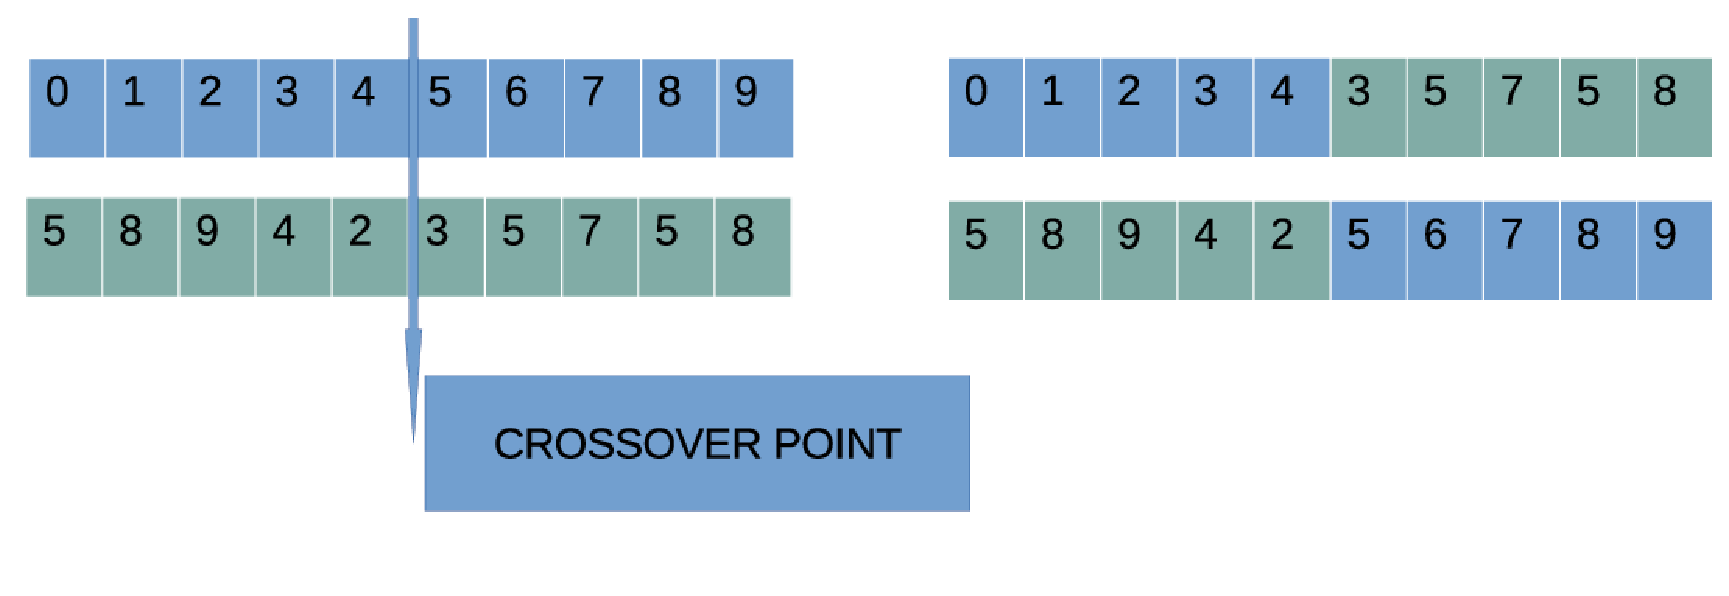
\includegraphics[scale=0.5]{onepoint_crossover}
\par\end{centering}
\caption{A graphical example of the one - point crossover. This procedure is
used in the Grammatical Evolution method to produce new chromosomes.\label{fig:onePoint}}
\end{figure}
\begin{figure}[H]
\begin{centering}
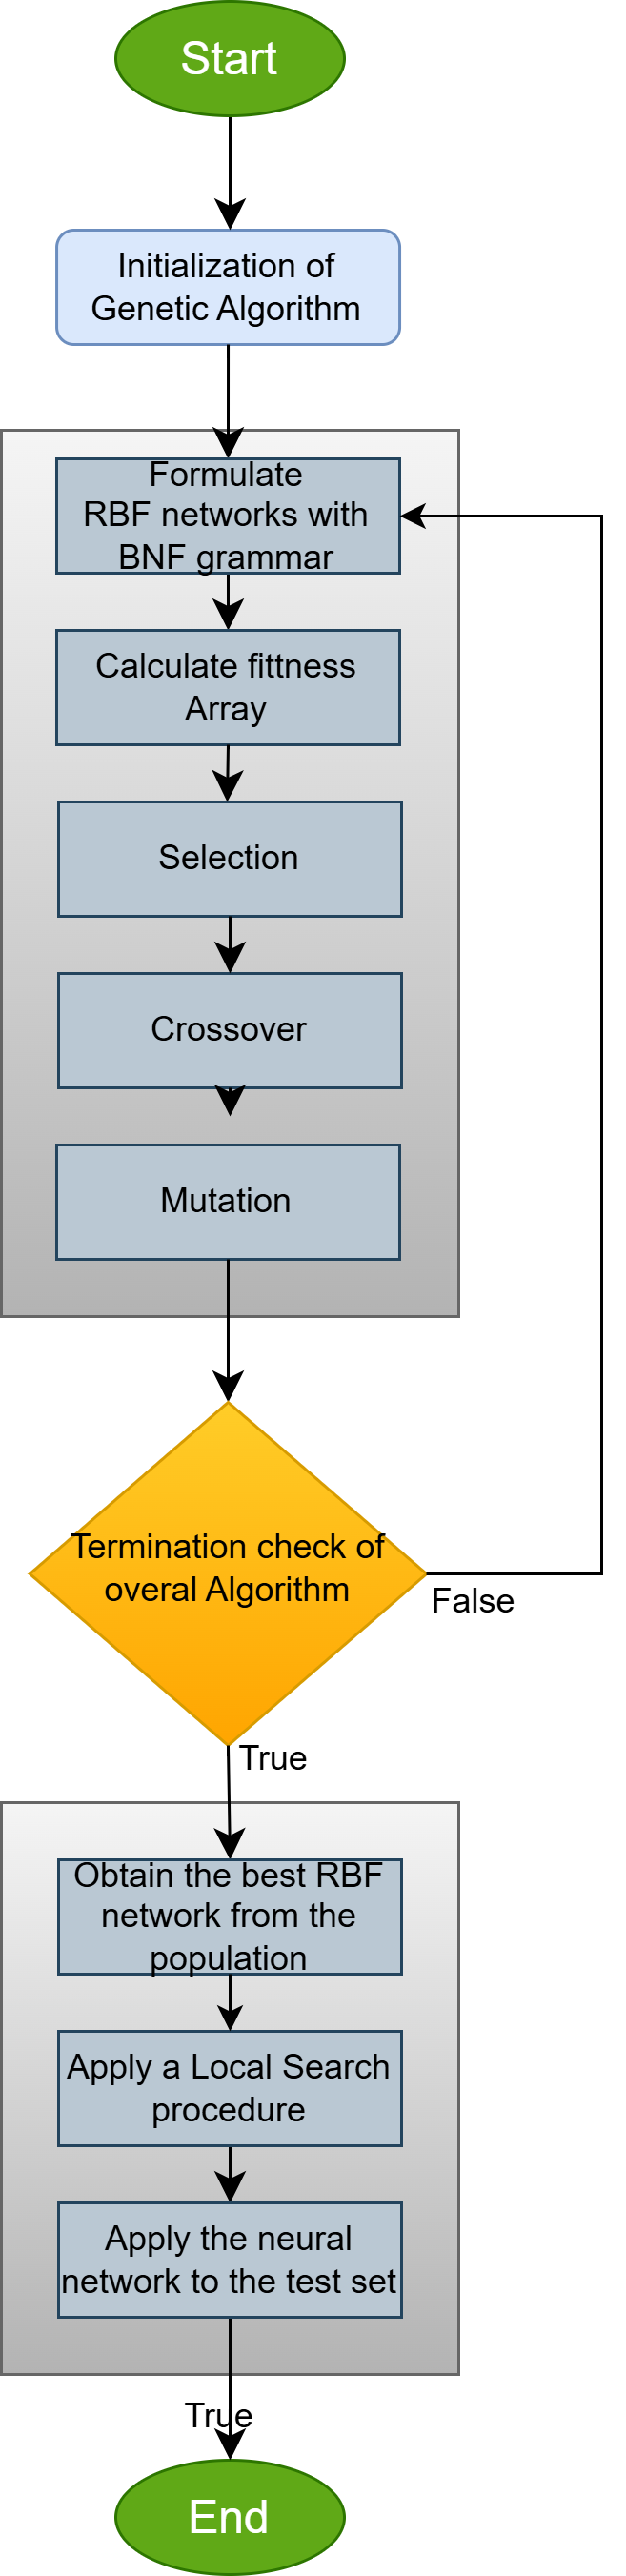
\includegraphics[scale=0.7]{flowchart}
\par\end{centering}
\caption{The steps of the proposed method as a flowchart.\label{fig:flow}}

\end{figure}


\subsection{Installation procedure}

The software was coded entirely in ANSI C++ and the software is available
freely from the following URL: \url{https://github.com/itsoulos/RbfCon}
(accessed on 14 November 2024). The user should install the QT Library,
which is accessible from \url{https://qt.io} (accessed on 14 November
2024) in order to compile the software. After downloading the RbfCon-master.zip
file, the user should execute the following commands, under any Unix
- based system:
\begin{enumerate}
\item unzip RbfCon-master.zip.
\item cd RbfCon-master
\item qmake (or qmake-qt5 in some Linux installations).
\item make
\end{enumerate}
For windows systems the user alternatively could install the software
using the RBFCON.msi located in the distribution, which is an installation
file that installs the software without the need for the QT Library.

\subsection{The main executable RbfCon}

The final outcome of the compilation has a series of command line
parameters, that the user may adjust. The list of this parameters
has as follows:
\begin{enumerate}
\item $--$trainfile=\textless filename\textgreater{} The string parameter
\emph{filename} determines the name of the file containing the training
dataset for the software. The user is required to provide this parameter
to start the process. The format for this file is shown in Figure
\ref{fig:datasetFormat}. The first number denoted as D in this figure
determines the dimension of the input dataset and the second number
denoted as M represents the number of input patterns. Every line in
the file contains a pattern and the required desired output.
\item $--$testfile=\textless filename\textgreater{} The string parameter
\emph{filename} stands for the name of the test dataset used by the
software. The user should provide at least the parameters \emph{trainfile}
and \emph{testfile} in order to initiate the method. The format of
the test dataset is the same as the training dataset.
\item $--$chromosome\_count=\textless count\textgreater{} This integer
parameter denotes the number of chromosomes in the genetic algorithm
(parameter $N_{c}$ of the algorithm). The default value for this
parameter is 500.
\item $--$chromosome\_size=\textless size\textgreater{} The integer parameter
\emph{size} determines the size of each chromosome for the Grammatical
Evolution process. The default value for this parameter is 100.
\item $--$selection\_rate=\textless rate\textgreater{} The double precision
parameter \emph{rate} stands for the selection rate of the Grammatical
Evolution process . The default value for this parameter is 0.10 (10\%).
\item $--$mutation\_rate=\textless rate\textgreater{} The double precision
parameter \emph{rate} represents the mutation rate for the Grammatical
Evolution process. The default value for this parameter is 0.05 (5\%).
\item $--$generations=\textless gens\textgreater{} The integer parameter
\emph{gens} stands for the maximum number of allowed generations for
the Grammatical Evolution procedure (parameter $N_{g}$ of the current
algorithm). The original value is 500.
\item $--$local\_method=\textless method\textgreater{} The used local
optimization method, that will be applied to the parameters of the
RBF model when the Grammatical Evolution procedure finished. The available
local optimization methods are:
\begin{enumerate}
\item \emph{lbfgs}. The method L-BFGS can be considered as a variation of
the Broyden--Fletcher--Goldfarb--Shanno (BFGS) optimization technique
\citep{bfgs2}, that utilizes a minimum amount of memory.\textbf{
}This optimization method has been used in many cases, such as image
reconstruction \citep{lbfgs_image},\textbf{ }inverse eigenvalue problems
\citep{lbfgs_inverse}, seismic problems \citep{lbfgs_seismic}, training
of deep neural networks \citep{lbfgs_deep}\textbf{ }etc.\textbf{
}Also, the a series of modifications have been proposed that take
advantage of modern parallel computing systems \citep{lbfgs_par1,lbfgs_par2,lbfgs_par3}.
\item \emph{bfgs}. The BFGS variant of Powell was used here \citep{powell},
when this option is enabled. 
\item \emph{adam}. This option denotes the application of the Adam optimizer
\citep{Adam} as the local optimization algorithm.
\item \emph{gradient}. This option represents the usage of the Gradient
Descent method \citep{GradientDescent} as the local optimization
algorithm.
\item \emph{none}. With this option no local optimization method will be
used after the Genetic Algorithm is terminated.
\end{enumerate}
\item $--$iterations=\textless iters\textgreater{} This integer parameter
determines the number of consecutive applications of the proposed
technique to the original data set. The default value is 30.
\end{enumerate}
\begin{figure}[H]
$ $

D

M

$\begin{array}{ccccc}
x_{11} & x_{12} & \ldots & x_{1D} & y_{1}\\
x_{21} & x_{22} & \ldots & x_{2D} & y_{2}\\
\vdots & \vdots & \vdots & \vdots & \vdots\\
x_{M1} & x_{M2} & \ldots & x_{MD} & y_{M}
\end{array}$

\caption{The format for the used datasets.\label{fig:datasetFormat}}
\end{figure}


\subsection{Example of execution}

As a full working example, consider the Wdbc dataset \citep{Wdbc}
which is located under EXAMPLES subdirectory. This dataset is used
for the detection of breast tumors. An example of execution could
be the following:

\inputencoding{latin9}\begin{lstlisting}[basicstyle={\scriptsize}]
./RbfCon --trainfile=EXAMPLES/wdbc.train --testfile=EXAMPLES/wdbc.test --iterations=2
\end{lstlisting}
\inputencoding{utf8}The output of this command is shown below:

\inputencoding{latin9}\begin{lstlisting}[basicstyle={\footnotesize},frame=single]
Iteration:    1 TRAIN ERROR:          20.40039584
Iteration:    1 TEST  ERROR:        0.07733519754
Iteration:    1 CLASS ERROR:                 9.12%
Iteration:    1 SOLUTION:    ((6.711)*(exp((-((pow(x13-(-97.73),2))+
  ((pow(x23-(43.7),2))+((pow(x23-(84.7),2))+
  (pow(x23-(91.3),2))))))/(2*pow((60.1),2))))+
  (-0.0099969))+((-0.39)*(exp((-((pow(x25-(9.336),2))+
  ((pow(x18-(6.8),2))+(pow(x4-(6.52),2)))))/(2*pow((711.5),2))))+
  (0.00185452))+((3.7)*(exp((-(pow(x3-(-6.8),2)))/(2*pow((2.3),2))))+
  (-0.001))+((-5.8)*(exp((-(pow(x2-(-99969.10),2)))/
  (2*pow((6342.3747),2))))+(-0.002))
Iteration:    2 TRAIN ERROR:          16.06705417
Iteration:    2 TEST  ERROR:        0.05654528154
Iteration:    2 CLASS ERROR:                 4.56%
Iteration:    2 SOLUTION:    ((4.4)*(exp((-((pow(x27-(3.6),2))+
  (pow(x23-(8.9893),2))))/(2*pow((49.9),2))))+(-0.004))+
  ((-2.09)*(exp((-((pow(x23-(-9.1),2))+
  ((pow(x30-(-40.4),2))+((pow(x4-(98.5),2))+
  (pow(x22-(-4.4),2))))))/(2*pow((189.9),2))))+(0.007))+
  ((-9.8)*(exp((-((pow(x2-(24.4),2))+((pow(x28-(2.04),2))+
  (pow(x27-(9.11),2)))))/(2*pow((3.1),2))))+(0.009))+
  ((-67.49)*(exp((-(pow(x10-(-2629940.4),2)))/(2*pow((098.5),2))))+(0.0094))
Average Train Error:          18.23372501
Average Test  Error:        0.06694023954
Average Class Error:                 6.84%
\end{lstlisting}
\inputencoding{utf8}The program prints the train error, the test error and the classification
for every run as well as the averages for these values. Also, in each
execution the main program shows the constructed RBF network as a
string value.

The basic elements that the software requires when initializing the
process are essentially the file containing the training data as well
as the file containing the test data. Both of these files must have
the proposed structure but also the same number of patterns. The user
can change other elements of the algorithm, such as the number of
chromosomes, through a series of parameters, but this is not required.
At the end, the software will display the average training error as
well as the average error in the test set as well as the average classification
error. 

\section{Results\label{sec:Results}}

The new technique can be used to construct RBF networks for both classification
and data fitting problems. For this reason, datasets covering many
scientific areas are used from the following websites:
\begin{enumerate}
\item The UCI repository, \url{https://archive.ics.uci.edu/}(accessed on
14 November 2024)\citep{uci}
\item The Keel repository, \url{https://sci2s.ugr.es/keel/datasets.php}(accessed
on 14 November 2024)\citep{Keel}.
\item The Statlib URL\textbf{ \url{ftp://lib.stat.cmu.edu/datasets/index.html }}(accessed
on 14 November 2024). 
\end{enumerate}

\subsection{The used datasets }

The following list contains the used classification datasets for the
the conducted experiments:
\begin{enumerate}
\item \textbf{Appendicitis}, a medical dataset that was studied in \citep{appendicitis,appendicitis2}.
This problem has 2 distinct classes.
\item \textbf{Alcohol}, a dataset related to alcohol consumption \citep{alcohol}.
This dataset contains 4 distinct classes.
\item \textbf{Australian}, an economic dataset \citep{australian}. The
number of classes for this dataset is 2.
\item \textbf{Bands}, related to problems occurred in printing \citep{bands}
and it has two classes.
\item \textbf{Cleveland}, a medical dataset proposed in a series of research
papers \citep{cleveland1,cleveland2}. This dataset has 5 distinct
classes.
\item \textbf{Dermatology}, which is also a medical dataset originated in
\citep{dermatology} and it has 6 classes.
\item \textbf{Ecoli}, that is related to problems regarding proteins \citep{ecoli}
and it has 8 classes.
\item \textbf{Fert}, used in demographics and it has two distinct classes.
\item \textbf{Haberman}, a medical dataset related to the detection of breast
cancer. This dataset has two classes.
\item \textbf{Hayes-roth} dataset \citep{hayes-roth}. This dataset has
3 classes.
\item \textbf{Heart}, a medical dataset about heart diseases \citep{heart}.
This dataset has two classes.
\item \textbf{HeartAttack}, which is a medical dataset related to heart
diseases having two distinct classes.
\item \textbf{Hepatitis}, a dataset used for the detection of hepatitis. 
\item \textbf{Housevotes}, used for the Congressional voting in USA \citep{housevotes}.
\item \textbf{Ionosphere}, used for measurements from the ionosphere \citep{ion1,ion2}
and it has two classes.
\item \textbf{Liverdisorder}, which is a medical dataset \citep{liver,liver1}
with two classes.
\item \textbf{Lymography} \citep{lymography}, that has 4 classes.
\item \textbf{Magic}, this dataset contains generated data to simulate registration
of high energy gamma particles \citep{magic} and it has two classes.
\item \textbf{Mammographic}, a medical dataset related to the presence of
breast cancer \citep{mammographic}.
\item \textbf{Parkinsons}, a dataset used for the detection of Parkinson's
disease \citep{parkinsons1,parkinsons2}.
\item \textbf{Pima}, a medical dataset that was useful for the detection
of diabetes \citep{pima}.
\item \textbf{Popfailures}, a dataset contains climate measurements \citep{popfailures}
and it has two classes.
\item \textbf{Regions2}, a medical dataset that contains measurements from
liver biopsy images \citep{regions2} and it has five classes.
\item \textbf{Ring}, which is a problem with 20 dimensions and two classes,
related to a series of multivariate normal distributions. 
\item \textbf{Saheart}, a medical dataset related to heart diseases with
2 classes \citep{saheart}.
\item \textbf{Statheart}, which is a also a medical dataset related to heart
diseases.
\item \textbf{Spambase}, a dataset used to detect spam emails from a large
database. The dataset has two distinct classes.
\item \textbf{Spiral}, an artificial dataset with two classes.
\item \textbf{Student}, a dataset contains measurements from various experiments
in schools \citep{student}.
\item \textbf{Tae}, this dataset consist of evaluations of teaching performance
and it has 3 classes.
\item \textbf{Transfusion}, which is a medical dataset \citep{transfusion}.
\item \textbf{Wdbc}, a medical dataset used to detect the presence of breast
cancer\citep{wdbc1,wdbc2}.
\item \textbf{Wine}, a dataset contains measurements about the quality of
wines \citep{wine1,wine2}, with 3 distinct classes.
\item \textbf{EEG} dataset, which is a medical dataset about EEG measurements
studied in a series of papers \citep{eeg1,eeg2}. The following cases
were obtained from this dataset: Z\_F\_S, ZO\_NF\_S, Z\_O\_N\_F\_S
and ZONF\_S.
\item \textbf{Zoo}, that used to detect the class of some animals \citep{zoo}
and it contains seven classes.
\end{enumerate}
The next list provided the regression datasets that was incorporated
during the conducted experiments:
\begin{enumerate}
\item \textbf{Abalone}, a dataset that used to predict the age of abalones
with 8 features.
\item \textbf{Airfoil}, a dataset provided by NASA \citep{airfoil} with
5 features.
\item \textbf{Auto}, a dataset used to predict the fuel consumption with
7 features.
\item \textbf{BK}, that contains measurements from a series of basketball
games and it has 4 features.
\item \textbf{BL}, a dataset used to record electricity experiments and
it contains 7 features.
\item \textbf{Baseball}, a dataset with 16 features used to estimate the
income of baseball players.
\item \textbf{Concrete}, a dataset with 8 features used in civil engineering
\citep{concrete}.
\item \textbf{DEE}, a dataset with 6 featured that was to predict the electricity
cost.
\item \textbf{FA}, that contains measurements about the body fat and it
has 18 features.
\item \textbf{HO}, a dataset originated in the STATLIB repository with 13
features.
\item \textbf{Housing}, used to predict the price of houses \citep{housing}
and it has 13 features.
\item \textbf{Laser}, which is a dataset with 4 features and it has been
used in various laser experiments.
\item \textbf{LW}, a dataset with 9 features used to record the weight of
babies.
\item \textbf{MB}, a dataset provide by from Smoothing Methods in Statistics
\citep{stat} with 2 features.
\item \textbf{Mortgage}, an economic dataset from USA with 15 features.
\item \textbf{NT}, a dataset with two features used to record body temperatures
\citep{ntdataset}.
\item \textbf{Plastic}, a dataset with 2 features used to detect the pressure
on plastics.
\item \textbf{PL}, a dataset with 2 features provided by the STATLIB repository.
\item \textbf{Quake}, a dataset used to measure the strength of earthquakes
with 3 features.
\item \textbf{SN}, a dataset that provides experimental measurements related
to trellising and pruning. This dataset has 11 features.
\item \textbf{Stock}, a dataset with 9 features used to approximate the
prices of various stocks.
\item \textbf{Treasury}, an economic dataset from USA that contains 15 features.
\item \textbf{TZ}, which is a dataset originated in the STATLIB repository
and it has 60 features.
\end{enumerate}

\subsection{Experimental results}

The implementation of the machine learning methods that participated
in the conducted experiments was made using ANSI C++. The experiments
were conducted 30 times and the average classification or regression
error as measured on the test was recorded.\textbf{ }The classification
error is measured as:
\begin{equation}
E_{C}\left(M(x)\right)=100\times\frac{\sum_{i=1}^{N}\left(\mbox{class}\left(M\left(x_{i}\right)\right)-y_{i}\right)}{N}
\end{equation}
where $M(x)$ denotes the used machine learning model and set $T$
denotes the train dataset.\textbf{ }On the other hand, the regression
error is calculated as: 
\begin{equation}
E_{R}\left(M(x)\right)=\frac{\sum_{i=1}^{N}\left(M\left(x_{i}\right)-y_{i}\right)^{2}}{N}
\end{equation}
The well - known technique of ten - fold cross validation was incorporated
for the validation of the experimental results. The experiments were
executed on an AMD Ryzen 5950X with 128GB of RAM, running as the operating
system the Debian Linux. The values for the parameters of the algorithm
are presented in Table \ref{tab:expValues}. 
\begin{table}[H]
\caption{The values for the experimental parameters.\label{tab:expValues}}

\centering{}%
\begin{tabular}{|c|c|}
\hline 
PARAMETER & VALUE\tabularnewline
\hline 
\hline 
chromosome\_count & 500\tabularnewline
\hline 
chromosome\_size & 100\tabularnewline
\hline 
selection\_rate & 0.1\tabularnewline
\hline 
mutation\_rate & 0.05\tabularnewline
\hline 
generations & 500\tabularnewline
\hline 
\end{tabular}
\end{table}
 This particular set of parameters has been used in a multitude of
scientific publications and can be considered as a compromise between
the efficiency of an evolutionary process such as the one proposed
in this work and the speed necessary to extract the results of its
application within a reasonable time. 

The experimental results from the application of various method on
the classification datasets are shown in Table \ref{tab:expClass}
and for the regression datasets in \ref{tab:expRegression}. For all
tables the following notation was used:
\begin{enumerate}
\item The column MLP(ADAM) represents the usage of the ADAM optimization
method \citep{Adam} to train an artificial neural network with $k=10$
processing nodes.
\item The column MLP(BFGS) stands for the usage of the BFGS optimization
method \citep{powell} in the training process of an artificial neural
network with $k=10$ processing nodes.
\item The column RBF denotes the usage of the original two - phase method
for the training of an RBF neural network with $k=10$ weights. This
method was described previously in subsection \ref{subsec:The-original-training}.
\item The column CRBF stands for the utilization of the current software
using the parameters of Table \ref{tab:expValues} and as local search
procedure the \emph{none} option was selected.
\item The column CRBF(LBFGS) denotes the application of the current method
using as local search procedure the L-Bfgs method.
\item The column CRBF(BFGS) stands for the application of the current work
using as local search procedure the Bfgs method.
\item The row denoted as AVERAGE, outlines the average classification or
regression error for all datasets in the corresponding table.
\item The row denoted as STDEV depicts the standard deviation for all datasets
in the corresponding table.
\end{enumerate}
\begin{table}[H]
\caption{Experimental results for the classification datasets using the mentioned
machine learning models.\label{tab:expClass}}

\raggedright{}%
\begin{tabular}{|c|c|c|c|c|c|c|}
\hline 
{\footnotesize{}DATASET} & {\footnotesize{}MLP(ADAM)} & {\footnotesize{}MLP(BFGS)} & {\footnotesize{}RBF} & {\footnotesize{}CRBF} & {\footnotesize{}CRBF(LBFGS)} & {\footnotesize{}CRBF(BFGS)}\tabularnewline
\hline 
\hline 
{\footnotesize{}APPENDICITIS} & {\footnotesize{}16.50\%} & {\footnotesize{}18.00\%} & {\footnotesize{}12.23\%} & {\footnotesize{}13.60\%} & {\footnotesize{}14.10\%} & {\footnotesize{}13.60\%}\tabularnewline
\hline 
{\footnotesize{}ALCOHOL} & {\footnotesize{}57.78\%} & {\footnotesize{}41.50\%} & {\footnotesize{}49.38\%} & {\footnotesize{}51.24\%} & {\footnotesize{}49.32\%} & {\footnotesize{}45.11\%}\tabularnewline
\hline 
{\footnotesize{}AUSTRALIAN} & {\footnotesize{}35.65\%} & {\footnotesize{}38.13\%} & {\footnotesize{}34.89\%} & {\footnotesize{}14.14\%} & {\footnotesize{}14.26\%} & {\footnotesize{}14.23\%}\tabularnewline
\hline 
{\footnotesize{}BANDS} & {\footnotesize{}36.92\%} & {\footnotesize{}36.67\%} & {\footnotesize{}37.17\%} & {\footnotesize{}35.75\%} & {\footnotesize{}36.58\%} & {\footnotesize{}36.03\%}\tabularnewline
\hline 
{\footnotesize{}CLEVELAND} & {\footnotesize{}67.55\%} & {\footnotesize{}77.55\%} & {\footnotesize{}67.10\%} & {\footnotesize{}49.14\%} & {\footnotesize{}49.52\%} & {\footnotesize{}50.28\%}\tabularnewline
\hline 
{\footnotesize{}DERMATOLOGY} & {\footnotesize{}26.14\%} & {\footnotesize{}52.92\%} & {\footnotesize{}62.34\%} & {\footnotesize{}45.20\%} & {\footnotesize{}38.43\%} & {\footnotesize{}36.66\%}\tabularnewline
\hline 
{\footnotesize{}ECOLI} & {\footnotesize{}64.43\%} & {\footnotesize{}69.52\%} & {\footnotesize{}59.48\%} & {\footnotesize{}54.18\%} & {\footnotesize{}54.39\%} & {\footnotesize{}53.03\%}\tabularnewline
\hline 
{\footnotesize{}FERT} & {\footnotesize{}23.98\%} & {\footnotesize{}23.20\%} & {\footnotesize{}15.00\%} & {\footnotesize{}15.20\%} & {\footnotesize{}15.50\%} & {\footnotesize{}15.90\%}\tabularnewline
\hline 
{\footnotesize{}HABERMAN} & {\footnotesize{}29.00\%} & {\footnotesize{}29.34\%} & {\footnotesize{}25.10\%} & {\footnotesize{}26.27\%} & {\footnotesize{}27.07\%} & {\footnotesize{}26.40\%}\tabularnewline
\hline 
{\footnotesize{}HAYES-ROTH} & {\footnotesize{}59.70\%} & {\footnotesize{}37.33\%} & {\footnotesize{}64.36\%} & {\footnotesize{}34.54\%} & {\footnotesize{}39.00\%} & {\footnotesize{}36.76\%}\tabularnewline
\hline 
{\footnotesize{}HEART} & {\footnotesize{}38.53\%} & {\footnotesize{}39.44\%} & {\footnotesize{}31.20\%} & {\footnotesize{}17.22\%} & {\footnotesize{}17.44\%} & {\footnotesize{}16.96\%}\tabularnewline
\hline 
{\footnotesize{}HEARTATTACK} & {\footnotesize{}45.55\%} & {\footnotesize{}46.67\%} & {\footnotesize{}29.00\%} & {\footnotesize{}22.60\%} & {\footnotesize{}21.83\%} & {\footnotesize{}21.53\%}\tabularnewline
\hline 
{\footnotesize{}HEPATITIS} & {\footnotesize{}68.13\%} & {\footnotesize{}72.47\%} & {\footnotesize{}64.63\%} & {\footnotesize{}54.25\%} & {\footnotesize{}47.50\%} & {\footnotesize{}48.75\%}\tabularnewline
\hline 
{\footnotesize{}HOUSEVOTES} & {\footnotesize{}7.48\%} & {\footnotesize{}7.13\%} & {\footnotesize{}6.13\%} & {\footnotesize{}3.05\%} & {\footnotesize{}3.65\%} & {\footnotesize{}3.05\%}\tabularnewline
\hline 
{\footnotesize{}IONOSPHERE} & {\footnotesize{}16.64\%} & {\footnotesize{}15.29\%} & {\footnotesize{}16.22\%} & {\footnotesize{}14.32\%} & {\footnotesize{}13.40\%} & {\footnotesize{}12.37\%}\tabularnewline
\hline 
{\footnotesize{}LIVERDISORDER} & {\footnotesize{}41.53\%} & {\footnotesize{}42.59\%} & {\footnotesize{}30.84\%} & {\footnotesize{}32.21\%} & {\footnotesize{}31.71\%} & {\footnotesize{}31.35\%}\tabularnewline
\hline 
{\footnotesize{}LYMOGRAPHY} & {\footnotesize{}39.79\%} & {\footnotesize{}35.43\%} & {\footnotesize{}25.50\%} & {\footnotesize{}26.36\%} & {\footnotesize{}25.71\%} & {\footnotesize{}21.49\%}\tabularnewline
\hline 
{\footnotesize{}MAGIC} & {\footnotesize{}40.55\%} & {\footnotesize{}17.30\%} & {\footnotesize{}21.28\%} & {\footnotesize{}22.18\%} & {\footnotesize{}19.62\%} & {\footnotesize{}20.35\%}\tabularnewline
\hline 
{\footnotesize{}MAMMOGRAPHIC} & {\footnotesize{}46.25\%} & {\footnotesize{}17.24\%} & {\footnotesize{}21.38\%} & {\footnotesize{}17.67\%} & {\footnotesize{}19.02\%} & {\footnotesize{}17.30\%}\tabularnewline
\hline 
{\footnotesize{}PARKINSONS} & {\footnotesize{}24.06\%} & {\footnotesize{}27.58\%} & {\footnotesize{}17.41\%} & {\footnotesize{}12.79\%} & {\footnotesize{}13.37\%} & {\footnotesize{}12.47\%}\tabularnewline
\hline 
{\footnotesize{}PIMA} & {\footnotesize{}34.85\%} & {\footnotesize{}35.59\%} & {\footnotesize{}25.78\%} & {\footnotesize{}24.13\%} & {\footnotesize{}24.90\%} & {\footnotesize{}24.15\%}\tabularnewline
\hline 
{\footnotesize{}POPFAILURES} & {\footnotesize{}5.18\%} & {\footnotesize{}5.24\%} & {\footnotesize{}7.04\%} & {\footnotesize{}6.98\%} & {\footnotesize{}6.94\%} & {\footnotesize{}6.80\%}\tabularnewline
\hline 
{\footnotesize{}REGIONS2} & {\footnotesize{}29.85\%} & {\footnotesize{}36.28\%} & {\footnotesize{}38.29\%} & {\footnotesize{}26.34\%} & {\footnotesize{}26.81\%} & {\footnotesize{}26.55\%}\tabularnewline
\hline 
{\footnotesize{}RING} & {\footnotesize{}28.80\%} & {\footnotesize{}29.24\%} & {\footnotesize{}21.67\%} & {\footnotesize{}11.08\%} & {\footnotesize{}10.13\%} & {\footnotesize{}10.33\%}\tabularnewline
\hline 
{\footnotesize{}SAHEART} & {\footnotesize{}34.04\%} & {\footnotesize{}37.48\%} & {\footnotesize{}32.19\%} & {\footnotesize{}29.52\%} & {\footnotesize{}29.28\%} & {\footnotesize{}29.19\%}\tabularnewline
\hline 
{\footnotesize{}SPAMBASE} & {\footnotesize{}48.05\%} & {\footnotesize{}18.16\%} & {\footnotesize{}29.35\%} & {\footnotesize{}16.95\%} & {\footnotesize{}15.53\%} & {\footnotesize{}15.60\%}\tabularnewline
\hline 
{\footnotesize{}SPIRAL} & {\footnotesize{}47.67\%} & {\footnotesize{}47.99\%} & {\footnotesize{}44.87\%} & {\footnotesize{}42.14\%} & {\footnotesize{}43.88\%} & {\footnotesize{}43.05\%}\tabularnewline
\hline 
{\footnotesize{}STATHEART} & {\footnotesize{}44.04\%} & {\footnotesize{}39.65\%} & {\footnotesize{}31.36\%} & {\footnotesize{}19.22\%} & {\footnotesize{}19.15\%} & {\footnotesize{}18.19\%}\tabularnewline
\hline 
{\footnotesize{}STUDENT} & {\footnotesize{}5.13\%} & {\footnotesize{}7.14\%} & {\footnotesize{}5.49\%} & {\footnotesize{}7.63\%} & {\footnotesize{}6.33\%} & {\footnotesize{}4.32\%}\tabularnewline
\hline 
{\footnotesize{}TAE} & {\footnotesize{}60.20\%} & {\footnotesize{}51.58\%} & {\footnotesize{}60.02\%} & {\footnotesize{}56.73\%} & {\footnotesize{}56.33\%} & {\footnotesize{}56.40\%}\tabularnewline
\hline 
{\footnotesize{}TRANSFUSION} & {\footnotesize{}25.68\%} & {\footnotesize{}25.84\%} & {\footnotesize{}26.41\%} & {\footnotesize{}25.15\%} & {\footnotesize{}24.70\%} & {\footnotesize{}24.36\%}\tabularnewline
\hline 
{\footnotesize{}WDBC} & {\footnotesize{}35.35\%} & {\footnotesize{}29.91\%} & {\footnotesize{}7.27\%} & {\footnotesize{}6.77\%} & {\footnotesize{}6.52\%} & {\footnotesize{}6.36\%}\tabularnewline
\hline 
{\footnotesize{}WINE} & {\footnotesize{}29.40\%} & {\footnotesize{}59.71\%} & {\footnotesize{}31.41\%} & {\footnotesize{}11.00\%} & {\footnotesize{}11.65\%} & {\footnotesize{}10.71\%}\tabularnewline
\hline 
{\footnotesize{}Z\_F\_S} & {\footnotesize{}47.81\%} & {\footnotesize{}39.37\%} & {\footnotesize{}13.16\%} & {\footnotesize{}11.13\%} & {\footnotesize{}11.47\%} & {\footnotesize{}10.57\%}\tabularnewline
\hline 
{\footnotesize{}Z\_O\_N\_F\_S} & {\footnotesize{}78.79\%} & {\footnotesize{}65.67\%} & {\footnotesize{}48.70\%} & {\footnotesize{}52.34\%} & {\footnotesize{}49.32\%} & {\footnotesize{}46.22\%}\tabularnewline
\hline 
{\footnotesize{}ZO\_NF\_S} & {\footnotesize{}47.43\%} & {\footnotesize{}43.04\%} & {\footnotesize{}9.02\%} & {\footnotesize{}11.08\%} & {\footnotesize{}11.18\%} & {\footnotesize{}8.90\%}\tabularnewline
\hline 
{\footnotesize{}ZONF\_S} & {\footnotesize{}11.99\%} & {\footnotesize{}15.62\%} & {\footnotesize{}4.03\%} & {\footnotesize{}4.14\%} & {\footnotesize{}3.94\%} & {\footnotesize{}3.58\%}\tabularnewline
\hline 
{\footnotesize{}ZOO} & {\footnotesize{}14.13\%} & {\footnotesize{}10.70\%} & {\footnotesize{}21.93\%} & {\footnotesize{}11.60\%} & {\footnotesize{}9.00\%} & {\footnotesize{}10.90\%}\tabularnewline
\hline 
\textbf{\footnotesize{}AVERAGE} & \textbf{\footnotesize{}37.23\%} & \textbf{\footnotesize{}35.36\%} & \textbf{\footnotesize{}30.23\%} & \textbf{\footnotesize{}24.63\%} & \textbf{\footnotesize{}24.17\%} & \textbf{\footnotesize{}23.42\%}\tabularnewline
\hline 
\textbf{\footnotesize{}STDEV} & \textbf{\footnotesize{}18.25\%} & \textbf{\footnotesize{}18.36\%} & \textbf{\footnotesize{}18.41\%} & \textbf{\footnotesize{}15.92\%} & \textbf{\footnotesize{}15.46\%} & \textbf{\footnotesize{}15.25\%}\tabularnewline
\hline 
\end{tabular}
\end{table}
\begin{table}[H]
\caption{Experimental results for the regression datasets using the series
of mentioned machine learning models.\label{tab:expRegression}}

\raggedright{}%
\begin{tabular}{|c|c|c|c|c|c|c|}
\hline 
{\footnotesize{}DATASET} & {\footnotesize{}MLP(ADAM)} & {\footnotesize{}MLP(BFGS)} & {\footnotesize{}RBF} & {\footnotesize{}CRBF} & {\footnotesize{}CRBF(LBFGS)} & {\footnotesize{}CRBF(BFGS)}\tabularnewline
\hline 
\hline 
{\footnotesize{}ABALONE} & {\footnotesize{}4.30} & {\footnotesize{}5.69} & {\footnotesize{}7.37} & {\footnotesize{}6.14} & {\footnotesize{}5.35} & {\footnotesize{}5.32}\tabularnewline
\hline 
{\footnotesize{}AIRFOIL} & {\footnotesize{}0.005} & {\footnotesize{}0.003} & {\footnotesize{}0.27} & {\footnotesize{}0.004} & {\footnotesize{}0.004} & {\footnotesize{}0.002}\tabularnewline
\hline 
{\footnotesize{}AUTO} & {\footnotesize{}70.84} & {\footnotesize{}60.97} & {\footnotesize{}17.87} & {\footnotesize{}11.03} & {\footnotesize{}10.03} & {\footnotesize{}9.45}\tabularnewline
\hline 
{\footnotesize{}BK} & {\footnotesize{}0.025} & {\footnotesize{}0.28} & {\footnotesize{}0.02} & {\footnotesize{}0.02} & {\footnotesize{}0.02} & {\footnotesize{}0.03}\tabularnewline
\hline 
{\footnotesize{}BL} & {\footnotesize{}0.62} & {\footnotesize{}2.55} & {\footnotesize{}0.013} & {\footnotesize{}0.04} & {\footnotesize{}0.024} & {\footnotesize{}0.01}\tabularnewline
\hline 
{\footnotesize{}BASEBALL} & {\footnotesize{}77.90} & {\footnotesize{}119.63} & {\footnotesize{}93.02} & {\footnotesize{}66.74} & {\footnotesize{}65.80} & {\footnotesize{}64.52}\tabularnewline
\hline 
{\footnotesize{}CONCRETE} & {\footnotesize{}0.078} & {\footnotesize{}0.066} & {\footnotesize{}0.011} & {\footnotesize{}0.012} & {\footnotesize{}0.010} & {\footnotesize{}0.009}\tabularnewline
\hline 
{\footnotesize{}DEE} & {\footnotesize{}0.63} & {\footnotesize{}2.36} & {\footnotesize{}0.17} & {\footnotesize{}0.23} & {\footnotesize{}0.22} & {\footnotesize{}0.20}\tabularnewline
\hline 
{\footnotesize{}FA} & {\footnotesize{}0.048} & {\footnotesize{}0.43} & {\footnotesize{}0.015} & {\footnotesize{}0.013} & {\footnotesize{}0.014} & {\footnotesize{}0.011}\tabularnewline
\hline 
{\footnotesize{}HO} & {\footnotesize{}0.035} & {\footnotesize{}0.62} & {\footnotesize{}0.03} & {\footnotesize{}0.013} & {\footnotesize{}0.015} & {\footnotesize{}0.012}\tabularnewline
\hline 
{\footnotesize{}HOUSING} & {\footnotesize{}81.00} & {\footnotesize{}97.38} & {\footnotesize{}57.68} & {\footnotesize{}20.60} & {\footnotesize{}19.02} & {\footnotesize{}18.40}\tabularnewline
\hline 
{\footnotesize{}LASER} & {\footnotesize{}0.03} & {\footnotesize{}0.015} & {\footnotesize{}0.03} & {\footnotesize{}0.06} & {\footnotesize{}0.05} & {\footnotesize{}0.03}\tabularnewline
\hline 
{\footnotesize{}LW} & {\footnotesize{}0.028} & {\footnotesize{}2.98} & {\footnotesize{}0.03} & {\footnotesize{}0.011} & {\footnotesize{}0.011} & {\footnotesize{}0.011}\tabularnewline
\hline 
{\footnotesize{}MB} & {\footnotesize{}0.06} & {\footnotesize{}0.129} & {\footnotesize{}5.43} & {\footnotesize{}0.055} & {\footnotesize{}0.06} & {\footnotesize{}0.12}\tabularnewline
\hline 
{\footnotesize{}MORTGAGE} & {\footnotesize{}9.24} & {\footnotesize{}8.23} & {\footnotesize{}1.45} & {\footnotesize{}0.165} & {\footnotesize{}0.18} & {\footnotesize{}0.074}\tabularnewline
\hline 
{\footnotesize{}NT} & {\footnotesize{}0.006} & {\footnotesize{}0.129} & {\footnotesize{}13.97} & {\footnotesize{}0.006} & {\footnotesize{}0.006} & {\footnotesize{}0.006}\tabularnewline
\hline 
{\footnotesize{}PLASTIC} & {\footnotesize{}11.71} & {\footnotesize{}20.32} & {\footnotesize{}8.62} & {\footnotesize{}3.58} & {\footnotesize{}2.86} & {\footnotesize{}2.43}\tabularnewline
\hline 
{\footnotesize{}PL} & {\footnotesize{}0.32} & {\footnotesize{}0.58} & {\footnotesize{}2.118} & {\footnotesize{}0.064} & {\footnotesize{}0.026} & {\footnotesize{}0.024}\tabularnewline
\hline 
{\footnotesize{}QUAKE} & {\footnotesize{}0.117} & {\footnotesize{}0.29} & {\footnotesize{}0.07} & {\footnotesize{}0.036} & {\footnotesize{}0.036} & {\footnotesize{}0.036}\tabularnewline
\hline 
{\footnotesize{}SN} & {\footnotesize{}0.026} & {\footnotesize{}0.4} & {\footnotesize{}0.027} & {\footnotesize{}0.025} & {\footnotesize{}0.026} & {\footnotesize{}0.025}\tabularnewline
\hline 
{\footnotesize{}STOCK} & {\footnotesize{}180.89} & {\footnotesize{}302.43} & {\footnotesize{}12.23} & {\footnotesize{}8.31} & {\footnotesize{}6.90} & {\footnotesize{}6.25}\tabularnewline
\hline 
{\footnotesize{}TREASURY} & {\footnotesize{}11.16} & {\footnotesize{}9.91} & {\footnotesize{}2.02} & {\footnotesize{}0.0027} & {\footnotesize{}0.12} & {\footnotesize{}0.10}\tabularnewline
\hline 
{\footnotesize{}TZ} & {\footnotesize{}0.43} & {\footnotesize{}0.22} & {\footnotesize{}0.036} & {\footnotesize{}0.036} & {\footnotesize{}0.036} & {\footnotesize{}0.035}\tabularnewline
\hline 
\textbf{\footnotesize{}AVERAGE} & \textbf{\footnotesize{}19.54} & \textbf{\footnotesize{}27.64} & \textbf{\footnotesize{}9.67} & \textbf{\footnotesize{}5.10} & \textbf{\footnotesize{}4.82} & \textbf{\footnotesize{}4.66}\tabularnewline
\hline 
\textbf{\footnotesize{}STDEV} & \textbf{\footnotesize{}43.67} & \textbf{\footnotesize{}68.11} & \textbf{\footnotesize{}22.01} & \textbf{\footnotesize{}14.34} & \textbf{\footnotesize{}14.05} & \textbf{\footnotesize{}13.76}\tabularnewline
\hline 
\end{tabular}
\end{table}


\section{Discussion\label{sec:Discussion}}

In Table \ref{tab:expClass}, for the APPENDICITIS dataset, the low
error rates of the RBF and CRBF models (12.23\% and 13.60\%, respectively)
indicate that Radial Basis Function-based models are well-suited for
this problem. This performance may be linked to their ability to handle
non-linear relationships in the data. The higher error rates of the
MLP models (above 16\%) suggest they might require more tuning or
larger datasets for optimal performance. In the ALCOHOL dataset, error
rates range from 41.50\% (MLP(BFGS)) to 57.78\% (MLP(ADAM)). This
wide variation implies that the dataset’s features are particularly
challenging for most models, likely due to noise or high dimensionality.
The intermediate error rates of the CRBF model (49.38\%) show that
while RBF-based models can handle some complexity, further adjustments
are needed to make them competitive. In the AUSTRALIAN dataset, CRBF
and its variations achieve exceptionally low error rates (14\%), highlighting
their strong adaptation to the dataset’s characteristics. In contrast,
MLP(ADAM) and MLP(BFGS) exhibit significantly higher errors (35\%-38\%),
demonstrating their struggles to perform effectively on this problem.
The CLEVELAND dataset, on the other hand, exemplifies complexity.
MLP models show error rates as high as 77.55\%, while CRBF models
reduce the error to about 49\%. This gap underscores the superiority
of RBF-based approaches for data with complex, non-linear structures.
Overall, the analysis reveals that CRBF models have a clear advantage
in datasets with non-linear relationships and lower dimensionality.
While MLP models are more flexible, they seem to require extensive
parameter tuning to achieve comparable performance. Employing an RBF
model with appropriate customization may often be the optimal choice
for many of the examined problems.

In Table \ref{tab:expRegression}, for the ABALONE dataset, MLP models
show higher values, such as 4.3 for MLP(ADAM) and 5.69 for MLP(BFGS),
while CRBF models perform better. The best result comes from CRBF(BFGS),
with a value of 5.32, indicating that CRBF models adapt better to
this dataset. In the AIRFOIL dataset, CRBF-based models exhibit exceptional
performance, with CRBF(BFGS) achieving the best value of 0.002. In
contrast, MLP models show higher values, such as 0.005 for MLP(ADAM),
demonstrating that RBF-based models are more accurate in this case.
In the AUTO dataset, there is a clear superiority of CRBF models.
CRBF(BFGS) achieves the best value of 9.45, while MLP models record
significantly higher values, such as 70.84 for MLP(ADAM). This indicates
that MLP struggles to adapt effectively to this problem. In the BASEBALL
dataset, CRBF models achieve lower error values, with the best result
being 64.52 for CRBF(BFGS). In comparison, MLP(ADAM) shows a much
higher value of 77.9, highlighting the advantage of CRBF models in
this dataset. In the HOUSING dataset, the differences are even more
pronounced. CRBF(BFGS) achieves the best performance with a value
of 18.4, while MLP(ADAM) records 81, and MLP(BFGS) reaches 97.38.
This stark contrast emphasizes the inability of MLP models to perform
effectively on this dataset. In the PLASTIC dataset, CRBF models also
deliver excellent performance. CRBF(BFGS) achieves the best result
at 2.43, while MLP models show much higher values, such as 11.71 for
MLP(ADAM). Overall, CRBF-based models demonstrate significantly lower
error values across most datasets, indicating their ability to adapt
to various data types. MLP models, although flexible, struggle in
many cases, possibly due to the need for extensive parameter tuning
or limitations in generalization. The overall analysis suggests that
CRBF models are more reliable for regression problems, especially
when the datasets involve non-linear relationships or high complexity.

Also, in Figures \ref{fig:statClass}, \ref{fig:statRegression} a
statistical comparison between all method is depicted.

\begin{figure}[H]
\begin{centering}
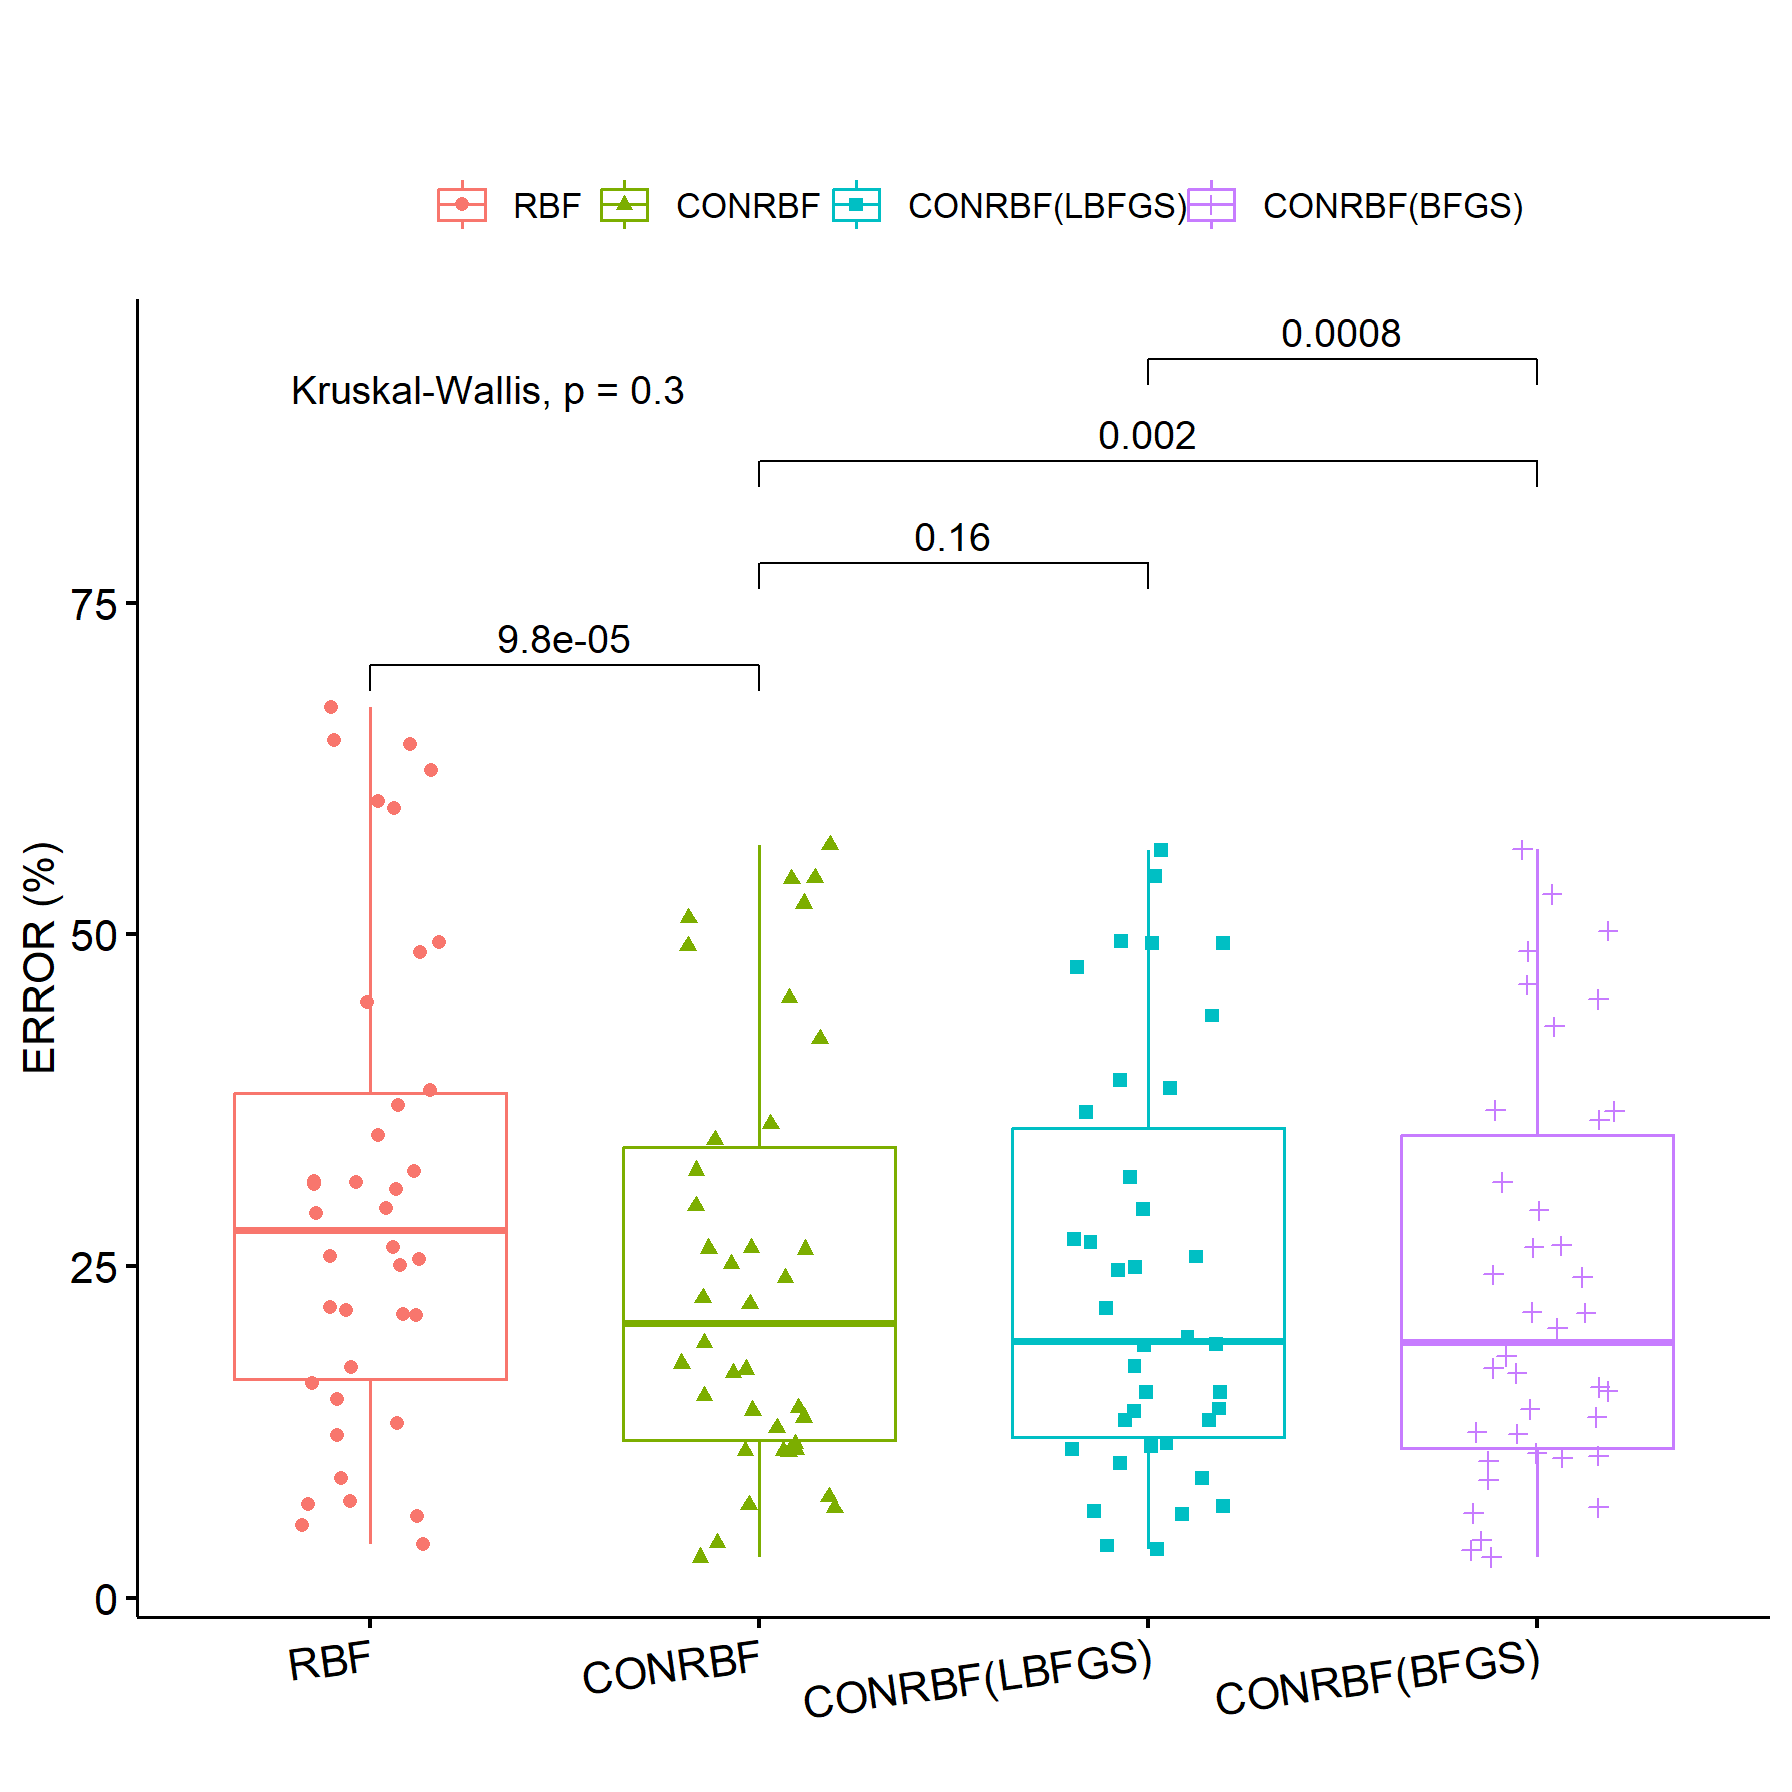
\includegraphics[scale=0.5]{t1}
\par\end{centering}
\caption{Statistical comparison for the used methods and the classification
datasets.\label{fig:statClass}}
\end{figure}
\begin{figure}[H]
\begin{centering}
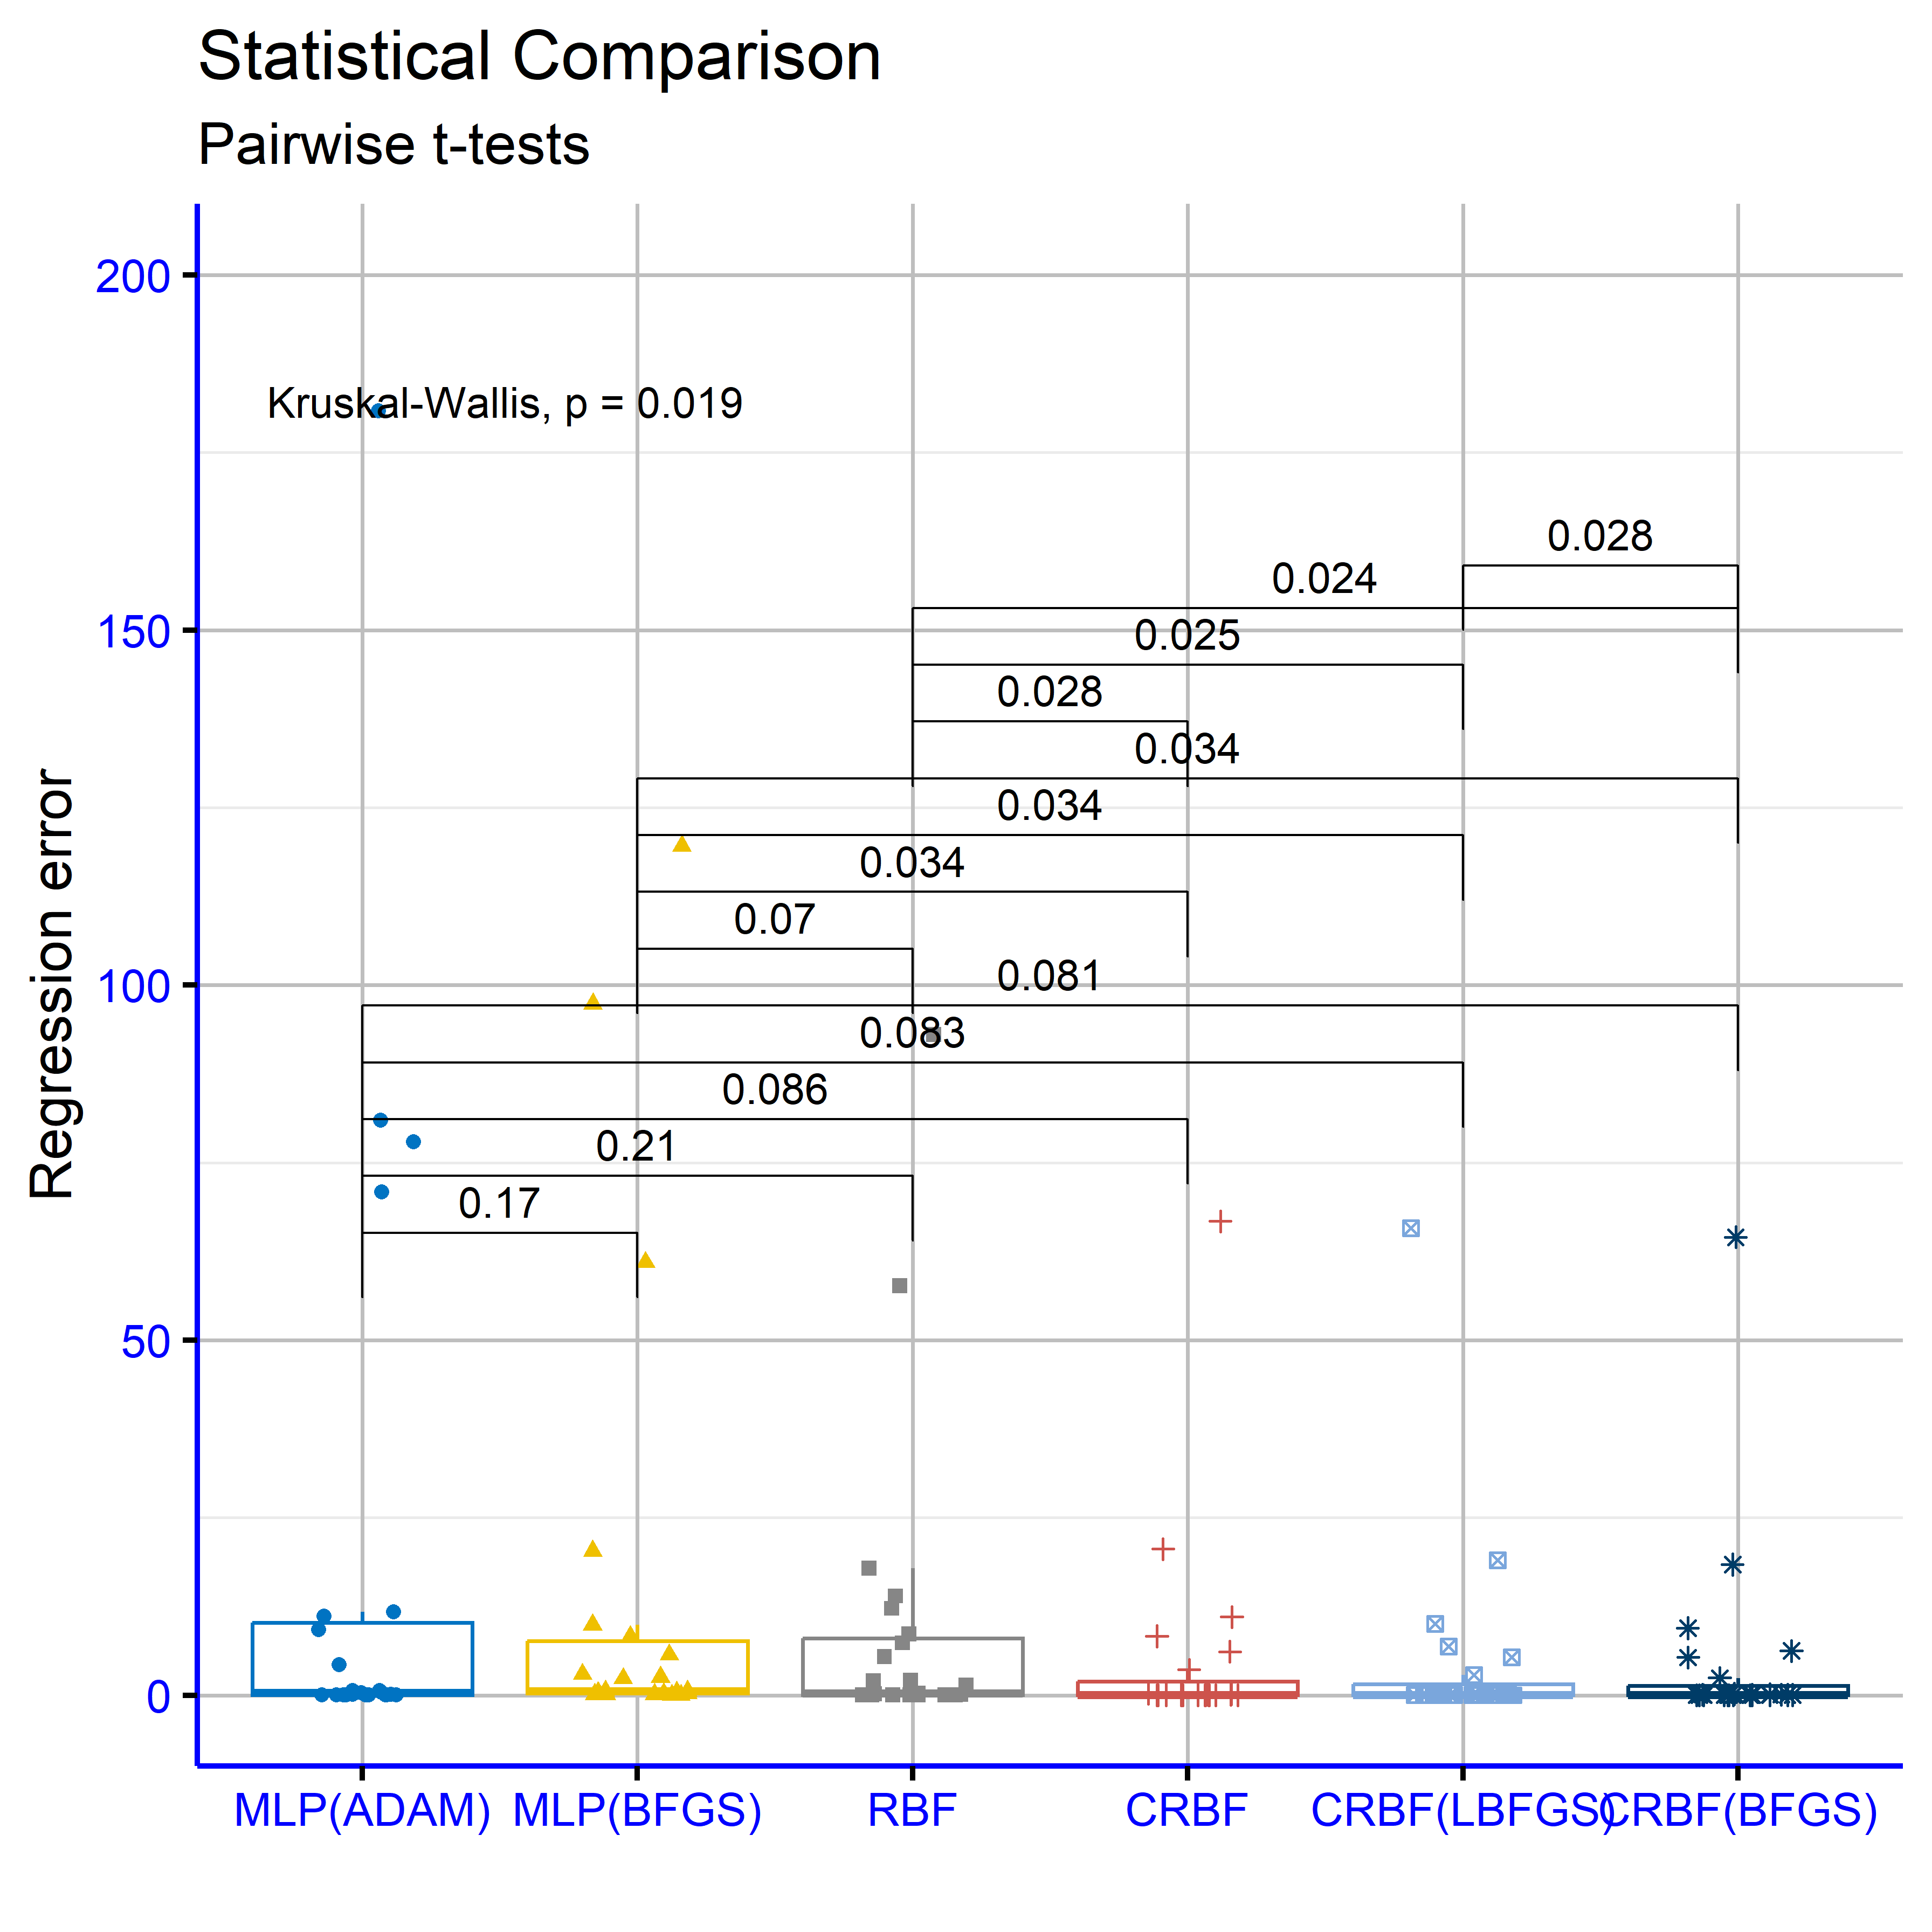
\includegraphics[scale=0.5]{t2}
\par\end{centering}
\caption{Statistical test for the regression datasets and the used methods.\label{fig:statRegression}}
\end{figure}
In Figure \ref{fig:statClass}, the Kruskal-Wallis test revealed statistically
significant differences among the methods overall, with a general
p-value of 0.0007, indicating that at least one method differs significantly
from the others in terms of classification error rates. Pairwise comparisons
provide further insights into the differences between specific methods.
The comparison between MLP(ADAM) and MLP(BFGS) showed no statistically
significant difference (p = 0.34), suggesting that the two methods
perform similarly. In contrast, the comparison between MLP(ADAM) and
RBF revealed a statistically significant difference (p = 0.0026),
indicating that RBF achieves distinct error rates compared to MLP(ADAM).
The comparison of MLP(ADAM) with CRBF showed a highly significant
difference (p = 1.8e-07), highlighting the superiority of CRBF over
MLP(ADAM). Similarly, the comparison between MLP(ADAM) and CRBF(LBFGS)
demonstrated even greater statistical significance, with p = 4.6e-08,
confirming the advantage of CRBF(LBFGS). Additionally, the comparison
of MLP(ADAM) with CRBF(BFGS) exhibited extremely high statistical
significance (p = 1.8e-08), favoring CRBF(BFGS). The subsequent comparisons
of MLP(BFGS) with other methods also revealed statistically significant
differences. The comparison between MLP(BFGS) and RBF yielded p =
0.011, indicating a notable difference, while the comparison of MLP(BFGS)
with CRBF had p = 3.8e-06, clearly demonstrating the superiority of
CRBF. Comparisons of MLP(BFGS) with CRBF(LBFGS) and CRBF(BFGS) resulted
in p-values of 1.9e-06 and 5.3e-07, respectively, confirming the statistical
significance of the differences. Furthermore, comparisons of RBF with
CRBF, CRBF(LBFGS), and CRBF(BFGS) all showed statistically significant
differences, with p-values of 9.8e-05, 3.9e-05, and 4.3e-06, respectively.
Finally, the comparison between CRBF(LBFGS) and CRBF(BFGS) also revealed
a statistically significant difference, with p = 0.0008. Overall,
the results demonstrate clear performance differences among the methods,
with CRBF consistently achieving superior results.

In Figure \ref{fig:statRegression}, The Kruskal-Wallis test revealed
statistically significant differences among the methods on regression
datasets, with an overall Kruskal-Wallis p-value of 0.0019. This indicates
that at least one method performs significantly differently from the
others. However, pairwise comparisons show mixed results. The comparison
between MLP(ADAM) and MLP(BFGS) did not show a statistically significant
difference (p = 0.17), suggesting similar performance between these
two methods. Similarly, the comparison between MLP(ADAM) and RBF was
not significant (p = 0.21). Comparisons of MLP(ADAM) with CRBF, CRBF(LBFGS),
and CRBF(BFGS) yielded p-values of 0.086, 0.083, and 0.081, respectively,
indicating trends toward differences but without statistical significance.
The comparisons involving MLP(BFGS) against other methods yielded
more pronounced results. Specifically, differences with CRBF, CRBF(LBFGS),
and CRBF(BFGS) were statistically significant, with p = 0.034 for
all three cases, indicating the superiority of the CRBF methods over
MLP(BFGS). For the comparisons between RBF and the CRBF methods, statistically
significant differences were observed. The comparison between RBF
and CRBF had a p-value of 0.028, while comparisons with CRBF(LBFGS)
and CRBF(BFGS) had p-values of 0.025 and 0.024, respectively, confirming
the superior performance of the CRBF methods. Finally, the comparison
between CRBF(LBFGS) and CRBF(BFGS) revealed a statistically significant
difference, with p = 0.028, highlighting a notable distinction in
the performance of these two methods. Overall, the results suggest
that while MLP methods perform similarly, CRBF methods consistently
achieve better results, with statistically significant differences
observed in most comparisons against the other methods.

Summarizing the above results, one can see that the proposed technique
for building and training RBF networks improves the performance of
these networks by more than 20\% on average on classification data
and by more than 50\% on regression data. In all datasets, the proposed
method brought about a significant reduction in classification error
in 80\% of cases and in many datasets the reduction in classification
or regression error was extremely significant. 

\section{Conclusions\label{sec:Conclusions}}

A novel method that constructs the architecture of RBF neural networks
with assistance was described in the present manuscript, accompanied
by the relevant software. The method can construct the architecture
of RBF networks using a process that incorporates the Grammatical
Evolution procedure. Also, the used method can estimate the parameters
of the network, which can be further modified by the application of
a local optimization procedure. The proposed method can be applied
without modifications to classification and regression datasets. The
new method was compared against the traditional method used to train
RBF networks and the experimental results validated the efficiency
of the proposed work in a wide series of classification and regression
datasets found in the recent bibliography.

The used software was coded in ANSI C++ with the assistance of the
freely available library of QT, in order to be portable on the majority
of operating systems. The user can control the process by a series
of simple command line options, such as the number of needed chromosomes
for the genetic population or the selection rate used. Also, the software
offers the possibility of improving the parameters of the RBF network
with the application of some local optimization procedures. The experimental
results  indicated that the application of the local optimization
algorithm can further reduce the test error in a series of datasets. 

Future improvements to the software may include the periodic application
of the local search procedure during the execution of the genetic
algorithm or even the incorporation of global optimization procedures,
in order to reduce even further the test error of the current work.
Also, since the method utilizes Genetic Algorithms, parallel optimization
procedures, such as MPI \citep{mpi} or OpenMP \citep{openmp} can
be used to reduce the execution time of the method. Finally, the software
could possibly be extended to allow the user to input other grammars
as parameters, or even to be able to use other output functions besides
Gaussian.

$ $

\authorcontributions{The proposed software was conceived and implemented by all members
of the team. The experiments were conducted using various classification
and regression datasets, and the comparative results were presented
by I.G.T and I.V. The statistical analysis was carried out by V.C.
All authors have reviewed and approved the final published version.}

\funding{This research received no external funding.}

\institutionalreview{Not Applicable.}

\informedconsent{Not applicable.}

\acknowledgments{This research has been financed by the European Union : Next Generation
EU through the Program Greece 2.0 National Recovery and Resilience
Plan , under the call RESEARCH -- CREATE -- INNOVATE, project name
“iCREW: Intelligent small craft simulator for advanced crew training
using Virtual Reality techniques\textquotedbl{} (project code:TAEDK-06195).}

\conflictsofinterest{The authors declare no conflicts of interest.}

\appendixtitles{no}

\begin{adjustwidth}{-\extralength}{0cm}{}

\reftitle{References}
\begin{thebibliography}{99}
\bibitem[(2006)]{physics-ml1} M. Mjahed, The use of clustering techniques
for the classification of high energy physics data, Nuclear Instruments
and Methods in Physics Research Section A: Accelerators, Spectrometers,
Detectors and Associated Equipment \textbf{559}, pp. 199-202, 2006.

\bibitem{physics_ml2}M Andrews, M Paulini, S Gleyzer, B Poczos, End-to-End
Event Classification of High-Energy Physics Data, Journal of Physics:
Conference Series \textbf{1085}, 2018.

\bibitem{chemistry_ml1}P. He, C.J. Xu, Y.Z. Liang, K.T. Fang, Improving
the classification accuracy in chemistry via boosting technique, Chemometrics
and Intelligent Laboratory Systems 70, pp. 39-46, 2004.

\bibitem{chemistry_ml2}J.A. Aguiar, M.L. Gong, T.Tasdizen, Crystallographic
prediction from diffraction and chemistry data for higher throughput
classification using machine learning, Computational Materials Science
\textbf{173}, 109409, 2020.

\bibitem{econ_ml1}I. Kaastra, M. Boyd, Designing a neural network
for forecasting financial and economic time series, Neurocomputing
\textbf{10}, pp. 215-236, 1996.

\bibitem{econ_ml2}R. Hafezi, J. Shahrabi, E. Hadavandi, A bat-neural
network multi-agent system (BNNMAS) for stock price prediction: Case
study of DAX stock price, Applied Soft Computing \textbf{29}, pp.
196-210, 2015.

\bibitem{med_ml1}S.S. Yadav, S.M. Jadhav, Deep convolutional neural
network based medical image classification for disease diagnosis.
J Big Data \textbf{6}, 113, 2019.

\bibitem{med_ml2}L. Qing, W. Linhong , D. Xuehai, A Novel Neural
Network-Based Method for Medical Text Classification, Future Internet
\textbf{11}, 255, 2019.

\bibitem[(1991)]{rbf1}J. Park and I. W. Sandberg, Universal Approximation
Using Radial-Basis-Function Networks, Neural Computation \textbf{3},
pp. 246-257, 1991.

\bibitem{rbf2}G.A. Montazer, D. Giveki, M. Karami, H. Rastegar, Radial
basis function neural networks: A review. Comput. Rev. J \textbf{1},
pp. 52-74, 2018.

\bibitem{bfgs2}R. Fletcher, A new approach to variable metric algorithms,
Computer Journal 13, pp. 317-322, 1970. 

\bibitem[(1991)]{rbfphysics1}V.I. Gorbachenko, M.V. Zhukov, Solving
boundary value problems of mathematical physics using radial basis
function networks. Comput. Math. and Math. Phys. \textbf{57}, pp.
145--155, 2017.

\bibitem[(1991)]{rbfphysics2}J. Määttä, V. Bazaliy, J. Kimari, F.
Djurabekova, K. Nordlund, T. Roos, Gradient-based training and pruning
of radial basis function networks with an application in materials
physics, Neural Networks \textbf{133}, pp. 123-131, 2021.

\bibitem[(1991)]{rbfrobotics1}R. -J. Lian, Adaptive Self-Organizing
Fuzzy Sliding-Mode Radial Basis-Function Neural-Network Controller
for Robotic Systems, IEEE Transactions on Industrial Electronics \textbf{61},
pp. 1493-1503, 2014.

\bibitem{rbfrobotics2}M. Vijay, D. Jena, Backstepping terminal sliding
mode control of robot manipulator using radial basis functional neural
networks. Computers \& Electrical Engineering \textbf{67}, pp. 690-707,
2018.

\bibitem[(1991)]{rbf_dos1}U. Ravale, N. Marathe, P. Padiya, Feature
Selection Based Hybrid Anomaly Intrusion Detection System Using K
Means and RBF Kernel Function, Procedia Computer Science \textbf{45},
pp. 428-435, 2015.

\bibitem{rbf_dos2}M. Lopez-Martin, A. Sanchez-Esguevillas, J. I.
Arribas, B. Carro, Network Intrusion Detection Based on Extended RBF
Neural Network With Offline Reinforcement Learning, IEEE Access \textbf{9},
pp. 153153-153170, 2021.

\bibitem[(1991)]{rbf_lmage1}Foody, G. M. (2004). Supervised image
classification by MLP and RBF neural networks with and without an
exhaustively defined set of classes. International Journal of Remote
Sensing, 25(15), 3091-3104.

\bibitem[(1991)]{rbf_image2}Er, M. J., Wu, S., Lu, J., \& Toh, H.
L. (2002). Face recognition with radial basis function (RBF) neural
networks. IEEE transactions on neural networks, 13(3), 697-710.

\bibitem[(1991)]{rbfinit1}L.I. Kuncheva, Initializing of an RBF network
by a genetic algorithm, Neurocomputing \textbf{14}, pp. 273-288, 1997.

\bibitem{rbfinit2}F. Ros, M. Pintore, A. Deman, J.R. Chrétien, Automatical
initialization of RBF neural networks, Chemometrics and Intelligent
Laboratory Systems \textbf{87}, pp. 26-32, 2007.

\bibitem{rbfinit3}D. Wang, X.J. Zeng, J.A. Keane, A clustering algorithm
for radial basis function neural network initialization, Neurocomputing
\textbf{77}, pp. 144-155, 2012.

\bibitem[(1991)]{rbfprun1}E. Ricci, R. Perfetti, Improved pruning
strategy for radial basis function networks with dynamic decay adjustment,
Neurocomputing \textbf{69}, pp. 1728-1732, 2006.

\bibitem{rbfprun3}Guang-Bin Huang, P. Saratchandran and N. Sundararajan,
A generalized growing and pruning RBF (GGAP-RBF) neural network for
function approximation, IEEE Transactions on Neural Networks \textbf{16},
pp. 57-67, 2005.

\bibitem{rbfprun2}M. Bortman and M. Aladjem, A Growing and Pruning
Method for Radial Basis Function Networks, IEEE Transactions on Neural
Networks \textbf{20}, pp. 1039-1045, 2009.

\bibitem[(1991)]{rbf_go1}Chen, J.Y.; Qin, Z.; Jia, J. A PSO-Based
Subtractive Clustering Technique for Designing RBF Neural Networks.
In Proceedings of the 2008 IEEE Congress on Evolutionary Computation
(IEEE World Congress on Computational Intelligence), Hong Kong, 1--6
June 2008; pp. 2047--2052. {[}Google Scholar{]}

\bibitem[(1991)]{rbf_go2}Esmaeili, A.; Mozayani, N. Adjusting the
parameters of radial basis function networks using Particle Swarm
Optimization. In Proceedings of the 2009 IEEE International Conference
on Computational Intelligence for Measurement Systems and Applications,
Hong Kong, 11--13 May 2009; pp. 179--181. {[}Google Scholar{]}

\bibitem[(1991)]{rbf_go3}O’Hora, B.; Perera, J.; Brabazon, A. Designing
Radial Basis Function Networks for Classification Using Differential
Evolution. In Proceedings of the 2006 IEEE International Joint Conference
on Neural Network Proceedings, Vancouver, BC, USA, 16--21 July 2006;
pp. 2932--2937.

\bibitem{rbfkernel}N. Benoudjit, M. Verleysen, On the Kernel Widths
in Radial-Basis Function Networks, Neural Processing Letters \textbf{18},
pp. 139--154, 2003.

\bibitem{rbfgen}J. Paetz, Reducing the number of neurons in radial
basis function networks with dynamic decay adjustment, Neurocomputing
\textbf{62}, pp. 79-91, 2004.

\bibitem{rbfcon}H. Yu, P. D. Reiner, T. Xie, T. Bartczak, B. M. Wilamowski,
An Incremental Design of Radial Basis Function Networks, IEEE Transactions
on Neural Networks and Learning Systems \textbf{25}, pp. 1793-1803,
2014.

\bibitem{rbfpso}A. Alexandridis, E. Chondrodima, H. Sarimveis, Cooperative
learning for radial basis function networks using particle swarm optimization,
Applied Soft Computing \textbf{49}, pp. 485-497, 2016.

\bibitem{rbflearn}R. Neruda, P. Kudova, Learning methods for radial
basis function networks, Future Generation Computer Systems \textbf{21},
pp. 1131--1142, 2005.

\bibitem{rbfpar1}R. Yokota, L.A. Barba, M. G. Knepley, PetRBF ---
A parallel O(N) algorithm for radial basis function interpolation
with Gaussians, Computer Methods in Applied Mechanics and Engineering
\textbf{199}, pp. 1793-1804, 2010.

\bibitem{rbfpar2}C. Lu, N. Ma, Z. Wang, Fault detection for hydraulic
pump based on chaotic parallel RBF network, EURASIP J. Adv. Signal
Process. \textbf{2011}, 49, 2011.

\bibitem[(1991)]{kmeans}MacQueen, J.: Some methods for classification
and analysis of multivariate observations, in: Proceedings of the
fifth Berkeley symposium on mathematical statistics and probability,
Vol. 1, No. 14, pp. 281-297, 1967. 

\bibitem[(1991)]{geMain}M. O’Neill, C. Ryan, Grammatical evolution,
IEEE Trans. Evol. Comput. \textbf{5,}pp. 349--358, 2001.

\bibitem[(1991)]{bnf1}J. W. Backus. The Syntax and Semantics of the
Proposed International Algebraic Language of the Zurich ACM-GAMM Conference.
Proceedings of the International Conference on Information Processing,
UNESCO, 1959, pp.125-132.

\bibitem[(1991)]{ge_trig}C. Ryan, M. O’Neill, J.J. Collins, Grammatical
evolution: Solving trigonometric identities, proceedings of Mendel.
Vol. 98. 1998.

\bibitem[(1991)]{ge_music}A.O. Puente, R. S. Alfonso, M. A. Moreno,
Automatic composition of music by means of grammatical evolution,
In: APL '02: Proceedings of the 2002 conference on APL: array processing
languages: lore, problems, and applications July 2002 Pages 148--155. 

\bibitem[(1991)]{ge_nn}Lídio Mauro Limade Campo, R. Célio Limã Oliveira,Mauro
Roisenberg, Optimization of neural networks through grammatical evolution
and a genetic algorithm, Expert Systems with Applications \textbf{56},
pp. 368-384, 2016.

\bibitem{ge_nn2}K. Soltanian, A. Ebnenasir, M. Afsharchi, Modular
Grammatical Evolution for the Generation of Artificial Neural Networks,
Evolutionary Computation \textbf{30}, pp 291--327, 2022.

\bibitem{lbfgs_image}H. Wang, H. Gemmeke, T. Hopp, J. Hesser, Accelerating
image reconstruction in ultrasound transmission tomography using L-BFGS
algorithm, In: Medical Imaging 2019: Ultrasonic Imaging and Tomography;
109550B (2019) https://doi.org/10.1117/12.2512654 Event: SPIE Medical
Imaging, 2019, San Diego, California, United States.

\bibitem[(1991)]{ge_pacman}E. Galván-López, J.M. Swafford, M. O’Neill,
A. Brabazon, Evolving a Ms. PacMan Controller Using Grammatical Evolution.
In: , et al. Applications of Evolutionary Computation. EvoApplications
2010. Lecture Notes in Computer Science, vol 6024. Springer, Berlin,
Heidelberg, 2010.

\bibitem{ge_supermario}N. Shaker, M. Nicolau, G. N. Yannakakis, J.
Togelius, M. O'Neill, Evolving levels for Super Mario Bros using grammatical
evolution, 2012 IEEE Conference on Computational Intelligence and
Games (CIG), 2012, pp. 304-31.

\bibitem[(1991)]{ge_credit}A. Brabazon, M. O'Neill, Credit classification
using grammatical evolution, Informatica \textbf{30.3}, 2006.

\bibitem{ge_intrusion}S. Şen, J.A. Clark. A grammatical evolution
approach to intrusion detection on mobile ad hoc networks, In: Proceedings
of the second ACM conference on Wireless network security, 2009.

\bibitem[(1991)]{ge_geva}M. O'Neill, E. Hemberg, C. Gilligan, E.
Bartley, J. McDermott, A. Brabazon, GEVA: grammatical evolution in
Java. ACM SIGEVOlution \textbf{3}, pp. 17-22, 2008.

\bibitem{ge_christiansen}A. Ortega, M. de la Cruz, M. Alfonseca,
Christiansen Grammar Evolution: Grammatical Evolution With Semantics,
IEEE Transactions on Evolutionary Computation \textbf{11}, pp. 77-90,
Feb. 2007.

\bibitem{ge_gramevol}F. Noorian, A.M. de Silva, P.H.W. Leong, gramEvol:
Grammatical Evolution in R, Journal of Statistical Software \textbf{71},
pp. 1--26, 2016.

\bibitem{ge_gelab}M.A. Raja, C. Ryan, GELAB - A Matlab Toolbox for
Grammatical Evolution. In: Yin, H., Camacho, D., Novais, P., Tallón-Ballesteros,
A. (eds) Intelligent Data Engineering and Automated Learning -- IDEAL
2018. IDEAL 2018. Lecture Notes in Computer Science(), vol 11315,
2018. Springer, Cham. https://doi.org/10.1007/978-3-030-03496-2\_22

\bibitem{ge_genclass}N.Anastasopoulos, I.G. Tsoulos, A. Tzallas,
GenClass: A parallel tool for data classification based on Grammatical
Evolution, SoftwareX \textbf{16}, 100830, 2021.

\bibitem{ge_qfc}I.G. Tsoulos, QFC: A Parallel Software Tool for Feature
Construction, Based on Grammatical Evolution, Algorithms \textbf{15},
295, 2022.

\bibitem[(1989)]{genetic1}D. Goldberg, Genetic Algorithms in Search,
Optimization and Machine Learning, Addison-Wesley Publishing Company,
Reading, Massachussets, 1989.

\bibitem{genetic2}Z. Michaelewicz, Genetic Algorithms + Data Structures
= Evolution Programs. Springer - Verlag, Berlin, 1996.

\bibitem{lbfgs_inverse}Z. Dalvand, M. Hajarian, Solving generalized
inverse eigenvalue problems via L-BFGS-B method, Inverse Problems
in Science and Engineering \textbf{28}, pp. 1719-1746, 2020.

\bibitem{lbfgs_seismic}Y. Rao, Y. Wang, Seismic waveform tomography
with shot-encoding using a restarted L-BFGS algorithm, Scientific
Reports \textbf{7}, pp. 1-9, 2017.

\bibitem[Yousefi(2022)]{lbfgs_deep}Yousefi, M., Martínez Calomardo,
Á. (2022). A Stochastic Modified Limited Memory BFGS for Training
Deep Neural Networks. In: Arai, K. (eds) Intelligent Computing. SAI
2022. Lecture Notes in Networks and Systems, vol 507. Springer, Cham.
https://doi.org/10.1007/978-3-031-10464-0\_2

\bibitem{lbfgs_par1}Y. Fei, G. Rong, B. Wang, W. Wang, Parallel L-BFGS-B
algorithm on GPU, Computers \& Graphics \textbf{40}, pp. 1-9, 2014.

\bibitem{lbfgs_par2}L. D'Amore, G. Laccetti, D. Romano, G. Scotti,
A. Murli, Towards a parallel component in a GPU--CUDA environment:
a case study with the L-BFGS Harwell routine, International Journal
of Computer Mathematics \textbf{92}, pp. 59-76, 2015.

\bibitem{lbfgs_par3}M.M. Najafabadi, T.M. Khoshgoftaar, F. Villanustre
et al, Large-scale distributed L-BFGS, J Big Data \textbf{4}, 22,
2017.

\bibitem{lbfgs_study}J.L. Morales, A numerical study of limited memory
BFGS methods, Applied Mathematics Letters \textbf{15}, pp. 481-487,
2002.

\bibitem[powell(1989)]{powell}M.J.D Powell, A Tolerant Algorithm
for Linearly Constrained Optimization Calculations, Mathematical Programming
\textbf{45}, pp. 547-566, 1989. 

\bibitem[Kingma(1989)]{Adam}D. P. Kingma, J. L. Ba, ADAM: a method
for stochastic optimization, in: Proceedings of the 3rd International
Conference on Learning Representations (ICLR 2015), pp. 1--15, 2015.

\bibitem[Amari(1989)]{GradientDescent}Amari, S. I. (1993). Backpropagation
and stochastic gradient descent method. Neurocomputing, 5(4-5), 185-196.

\bibitem[Wolberg(1989)]{Wdbc}W.H. Wolberg, O.L. Mangasarian, Multisurface
method of pattern separation for medical diagnosis applied to breast
cytology, Proc Natl Acad Sci U S A. \textbf{87}, pp. 9193--9196,
1990.

\bibitem[(1989)]{uci}M. Kelly, R. Longjohn, K. Nottingham, The UCI
Machine Learning Repository, https://archive.ics.uci.edu.

\bibitem{Keel}J. Alcalá-Fdez, A. Fernandez, J. Luengo, J. Derrac,
S. García, L. Sánchez, F. Herrera. KEEL Data-Mining Software Tool:
Data Set Repository, Integration of Algorithms and Experimental Analysis
Framework. Journal of Multiple-Valued Logic and Soft Computing 17,
pp. 255-287, 2011.

\bibitem[Weiss(1989)]{appendicitis}Weiss, Sholom M. and Kulikowski,
Casimir A., Computer Systems That Learn: Classification and Prediction
Methods from Statistics, Neural Nets, Machine Learning, and Expert
Systems, Morgan Kaufmann Publishers Inc, 1991.

\bibitem{appendicitis2}M. Wang, Y.Y. Zhang, F. Min, Active learning
through multi-standard optimization, IEEE Access \textbf{7}, pp. 56772--56784,
2019.

\bibitem[Tzimourta(2018)]{alcohol}Tzimourta, K.D.; Tsoulos, I.; Bilero,
I.T.; Tzallas, A.T.; Tsipouras, M.G.; Giannakeas, N. Direct Assessment
of Alcohol Consumption in Mental State Using Brain Computer Interfaces
and Grammatical Evolution. Inventions 2018, 3, 51.

\bibitem[Quinlan(2018)]{australian}J.R. Quinlan, Simplifying Decision
Trees. International Journal of Man-Machine Studies \textbf{27}, pp.
221-234, 1987. 

\bibitem[Evans(1994)]{bands}B. Evans, D. Fisher, Overcoming process
delays with decision tree induction. IEEE Expert \textbf{9}, pp. 60-66,
1994.

\bibitem[(2004)]{cleveland1}Z.H. Zhou,Y. Jiang, NeC4.5: neural ensemble
based C4.5,\textquotedbl{} in IEEE Transactions on Knowledge and Data
Engineering \textbf{16}, pp. 770-773, 2004.

\bibitem{cleveland2}R. Setiono , W.K. Leow, FERNN: An Algorithm for
Fast Extraction of Rules from Neural Networks, Applied Intelligence
\textbf{12}, pp. 15-25, 2000.

\bibitem[(1998)]{dermatology}G. Demiroz, H.A. Govenir, N. Ilter,
Learning Differential Diagnosis of Eryhemato-Squamous Diseases using
Voting Feature Intervals, Artificial Intelligence in Medicine. \textbf{13},
pp. 147--165, 1998.

\bibitem[(1996)]{ecoli}P. Horton, K.Nakai, A Probabilistic Classification
System for Predicting the Cellular Localization Sites of Proteins,
In: Proceedings of International Conference on Intelligent Systems
for Molecular Biology \textbf{4}, pp. 109-15, 1996.

\bibitem[(1977)]{hayes-roth}B. Hayes-Roth, B., F. Hayes-Roth. Concept
learning and the recognition and classification of exemplars. Journal
of Verbal Learning and Verbal Behavior \textbf{16}, pp. 321-338, 1977.

\bibitem[(1997)]{heart}I. Kononenko, E. Šimec, M. Robnik-Šikonja,
Overcoming the Myopia of Inductive Learning Algorithms with RELIEFF,
Applied Intelligence \textbf{7}, pp. 39--55, 1997

\bibitem[(2002)]{housevotes}R.M. French, N. Chater, Using noise to
compute error surfaces in connectionist networks: a novel means of
reducing catastrophic forgetting, Neural Comput. \textbf{14}, pp.
1755-1769, 2002.

\bibitem[(2004)]{ion1}J.G. Dy , C.E. Brodley, Feature Selection for
Unsupervised Learning, The Journal of Machine Learning Research \textbf{5},
pp 845--889, 2004.

\bibitem{ion2}S. J. Perantonis, V. Virvilis, Input Feature Extraction
for Multilayered Perceptrons Using Supervised Principal Component
Analysis, Neural Processing Letters \textbf{10}, pp 243--252, 1999.

\bibitem[(2002)]{liver} J. Garcke, M. Griebel, Classification with
sparse grids using simplicial basis functions, Intell. Data Anal.
\textbf{6}, pp. 483-502, 2002.

\bibitem{liver1}J. Mcdermott, R.S. Forsyth, Diagnosing a disorder
in a classification benchmark, Pattern Recognition Letters \textbf{73},
pp. 41-43, 2016.

\bibitem[(2002)]{lymography}G. Cestnik, I. Konenenko, I. Bratko,
Assistant-86: A Knowledge-Elicitation Tool for Sophisticated Users.
In: Bratko, I. and Lavrac, N., Eds., Progress in Machine Learning,
Sigma Press, Wilmslow, pp. 31-45, 1987. 

\bibitem[(2002)]{magic}Heck, D., Knapp, J., Capdevielle, J. N., Schatz,
G., \& Thouw, T. (1998). CORSIKA: A Monte Carlo code to simulate extensive
air showers.

\bibitem[(2007)]{mammographic}M. Elter, R. Schulz-Wendtland, T. Wittenberg,
The prediction of breast cancer biopsy outcomes using two CAD approaches
that both emphasize an intelligible decision process, Med Phys. \textbf{34},
pp. 4164-72, 2007.

\bibitem[(2007)]{parkinsons1}M.A. Little, P.E. McSharry, S.J Roberts
et al, Exploiting Nonlinear Recurrence and Fractal Scaling Properties
for Voice Disorder Detection. BioMed Eng OnLine \textbf{6}, 23, 2007.

\bibitem{parkinsons2}M.A. Little, P.E. McSharry, E.J. Hunter, J.
Spielman, L.O. Ramig, Suitability of dysphonia measurements for telemonitoring
of Parkinson's disease. IEEE Trans Biomed Eng. \textbf{56}, pp. 1015-1022,
2009.

\bibitem[(2007)]{pima}J.W. Smith, J.E. Everhart, W.C. Dickson, W.C.
Knowler, R.S. Johannes, Using the ADAP learning algorithm to forecast
the onset of diabetes mellitus, In: Proceedings of the Symposium on
Computer Applications and Medical Care IEEE Computer Society Press,
pp.261-265, 1988.

\bibitem[(2007)]{popfailures}D.D. Lucas, R. Klein, J. Tannahill,
D. Ivanova, S. Brandon, D. Domyancic, Y. Zhang, Failure analysis of
parameter-induced simulation crashes in climate models, Geoscientific
Model Development \textbf{6}, pp. 1157-1171, 2013.

\bibitem[(2007)]{regions2}N. Giannakeas, M.G. Tsipouras, A.T. Tzallas,
K. Kyriakidi, Z.E. Tsianou, P. Manousou, A. Hall, E.C. Karvounis,
V. Tsianos, E. Tsianos, A clustering based method for collagen proportional
area extraction in liver biopsy images (2015) Proceedings of the Annual
International Conference of the IEEE Engineering in Medicine and Biology
Society, EMBS, 2015-November, art. no. 7319047, pp. 3097-3100. 

\bibitem[(2007)]{saheart}T. Hastie, R. Tibshirani, Non-parametric
logistic and proportional odds regression, JRSS-C (Applied Statistics)
\textbf{36}, pp. 260--276, 1987.

\bibitem[(2007)]{student}P. Cortez, A. M. Gonçalves Silva, Using
data mining to predict secondary school student performance, In Proceedings
of 5th FUture BUsiness TEChnology Conference (FUBUTEC 2008) (pp. 5--12).
EUROSIS-ETI, 2008.

\bibitem[(2007)]{transfusion}I-Cheng Yeh, King-Jang Yang, Tao-Ming
Ting, Knowledge discovery on RFM model using Bernoulli sequence, Expert
Systems with Applications \textbf{36}, pp. 5866-5871, 2009.

\bibitem[(2007)]{wdbc1}Jeyasingh, S., \& Veluchamy, M. (2017). Modified
bat algorithm for feature selection with the wisconsin diagnosis breast
cancer (WDBC) dataset. Asian Pacific journal of cancer prevention:
APJCP, 18(5), 1257.

\bibitem[(2007)]{wdbc2}Alshayeji, M. H., Ellethy, H., \& Gupta, R.
(2022). Computer-aided detection of breast cancer on the Wisconsin
dataset: An artificial neural networks approach. Biomedical signal
processing and control, 71, 103141.

\bibitem[(2007)]{wine1}M. Raymer, T.E. Doom, L.A. Kuhn, W.F. Punch,
Knowledge discovery in medical and biological datasets using a hybrid
Bayes classifier/evolutionary algorithm. IEEE transactions on systems,
man, and cybernetics. Part B, Cybernetics : a publication of the IEEE
Systems, Man, and Cybernetics Society, \textbf{33} , pp. 802-813,
2003.

\bibitem{wine2}P. Zhong, M. Fukushima, Regularized nonsmooth Newton
method for multi-class support vector machines, Optimization Methods
and Software \textbf{22}, pp. 225-236, 2007.

\bibitem[(2007)]{eeg1}R. G. Andrzejak, K. Lehnertz, F.Mormann, C.
Rieke, P. David, and C. E. Elger, “Indications of nonlinear deterministic
and finite-dimensional structures in time series of brain electrical
activity: dependence on recording region and brain state,” Physical
Review E, vol. 64, no. 6, Article ID 061907, 8 pages, 2001. 

\bibitem{eeg2}A. T. Tzallas, M. G. Tsipouras, and D. I. Fotiadis,
“Automatic Seizure Detection Based on Time-Frequency Analysis and
Artificial Neural Networks,” Computational Intelligence and Neuroscience,
vol. 2007, Article ID 80510, 13 pages, 2007. doi:10.1155/2007/80510

\bibitem[(2007)]{zoo}M. Koivisto, K. Sood, Exact Bayesian Structure
Discovery in Bayesian Networks, The Journal of Machine Learning Research\textbf{
5}, pp. 549--573, 2004.

\bibitem[(2007)]{abalone}Nash, W.J.; Sellers, T.L.; Talbot, S.R.;
Cawthor, A.J.; Ford, W.B. The Population Biology of Abalone (\_Haliotis\_
species) in Tasmania. I. Blacklip Abalone (\_H. rubra\_) from the
North Coast and Islands of Bass Strait, Sea Fisheries Division; Technical
Report No. 48; Department of Primary Industry and Fisheries, Tasmania:
Hobart, Australia, 1994; ISSN 1034-3288

\bibitem[(2007)]{airfoil}Brooks, T.F.; Pope, D.S.; Marcolini, A.M.
Airfoil Self-Noise and Prediction. Technical Report, NASA RP-1218.
July 1989. Available online: https://ntrs.nasa.gov/citations/19890016302
(accessed on 14 November 2024).

\bibitem[(2007)]{concrete}I.Cheng Yeh, Modeling of strength of high
performance concrete using artificial neural networks, Cement and
Concrete Research. \textbf{28}, pp. 1797-1808, 1998. 

\bibitem[(2007)]{housing}D. Harrison and D.L. Rubinfeld, Hedonic
prices and the demand for clean ai, J. Environ. Economics \& Management
\textbf{5}, pp. 81-102, 1978.

\bibitem[(2007)]{stat}Simonoff, J.S. Smooting Methods in Statistics;
Springer: Berlin/Heidelberg, Germany, 1996. 

\bibitem[(2007)]{ntdataset}Mackowiak, P.A.; Wasserman, S.S.; Levine,
M.M. A critical appraisal of 98.6 degrees f, the upper limit of the
normal body temperature, and other legacies of Carl Reinhold August
Wunderlich. J. Am. Med. Assoc. 1992, 268, 1578--1580.

\bibitem[(1996)]{mpi}Gropp, W.; Lusk, E.; Doss, N.; Skjellum, A.
A high-performance, portable implementation of the MPI message passing
interface standard. Parallel Comput. 1996, 22, 789--828.

\bibitem[(1996)]{openmp}Chandra, R. Parallel Programming in OpenMP;
Morgan Kaufmann: Cambridge, MA, USA, 2001.

\end{thebibliography}

\end{adjustwidth}{}
\end{document}
